%%
%% $Id: article.tex,v 1.1 2008/09/20 10:19:28 natalie Exp $
%% $Source: /Users/natalie/cvs/tex/templates/article.tex,v $
%% $Date: 2008/09/20 10:19:28 $
%% $Revision: 1.1 $
%%

%\documentclass[a4paper,11pt,BCOR1cm,DIV11,headinclude]{scrbook}
% bei 12pt ist DIV 12 default, bei 11pt ist es DIV 10
% Textbereiche 
% DIV 10: 147*207.9mm, DIV 11: 152.73*216mm, DIV 12:157.50*222.75
% DIV 13: 161.54*228.46mm, DIV 14: 165*233.36mm

\def\deftitle{Notes on hedging cryptos with spectral risk measures}
% \def\defauthor{N.\ Packham}
% \def\defauthor{nat}
\def\defauthor{}

%% option: largefont
\documentclass[square]{article} %
%% options: vscreen, garamond, wnotes, savespace
\usepackage[vscreen]{nat}
\usepackage[longnamesfirst]{natbib}
\usepackage{booktabs}

\bibpunct{(}{)}{;}{a}{,}{,}
\usepackage{amsfonts,amssymb,amsthm} %
\usepackage{mathrsfs}
\usepackage[tbtags]{amsmath} %
\usepackage{bm}
\usepackage{tabularx,ragged2e}
\usepackage[table,xcdraw]{xcolor}
\usepackage{subfig}

\newcolumntype{C}{>{\Centering\arraybackslash}X}
\newcolumntype{s}{>{\hsize=.2\hsize \Centering\arraybackslash}X}
% \usepackage{fullpage}
\usepackage{footnote}
\makesavenoteenv{tabular}

\usepackage{graphicx,color}
\graphicspath{{./pics/}}
\definecolor{BrickRed}{rgb}{.625,.25,.25}
\providecommand{\red}[1]{\textcolor{BrickRed}{#1}}
\definecolor{markergreen}{rgb}{0.6, 1.0, 0}
\definecolor{darkgreen}{rgb}{0, .5, 0}
\definecolor{darkred}{rgb}{.7,0,0}
\definecolor{markergreen}{rgb}{0.6, 1.0, 0}
\definecolor{darkgreen}{rgb}{0, .5, 0}
\definecolor{darkorange}{rgb}{1,0.3,0}
\definecolor{darkred}{RGB}{.7,0,0}
\definecolor{darkblue}{RGB}{0,29,245}
\definecolor{orange}{RGB}{239, 133, 54}
\definecolor{lightblue}{RGB}{59, 188, 175}

\providecommand{\marker}[1]{\fcolorbox{markergreen}{markergreen}{{#1}}}
\providecommand{\natp}[1]{\textcolor{darkred}{#1}}
\providecommand{\mj}[1]{\textcolor{darkred}{#1}}
\providecommand{\francis}[1]{\textcolor{darkgreen}{#1}}

\theoremstyle{plain}
\newtheorem{theorem}{Theorem}%[section]
\newtheorem{proposition}[theorem]{Proposition}
\newtheorem{corollary}[theorem]{Corollary} %%
\newtheorem{lemma}[theorem]{Lemma} %%
\theoremstyle{definition} %%
\newtheorem{definition}{Definition}
\newtheorem{remark}[theorem]{Remark}
\newtheorem{remarks}{Remarks}
\newtheorem{condition}[theorem]{Condition}
\newtheorem{example}[theorem]{Example}
\newtheorem{assumption}{Assumption}
\setlength{\parindent}{0pt}

\usepackage[makestderr]{pythontex}
\usepackage{amsmath}
\begin{pycode}
import numpy as np
from scipy import stats
import statsmodels.api as sm
import pandas as pd
import matplotlib.pyplot as plt
np.random.seed(87654)
\end{pycode}


\input{definitions}
\sloppy
\begin{document}
\setlength{\boxlength}{0.95\textwidth} %
\title{\large{\bf\deftitle}} %
\author{{\normalsize\bf\defauthor}}%
\thispagestyle{empty}
\addtocounter{page}{1}
\maketitle
\begin{abstract}
  We investigate different methods of hedging cryptocurrencies with
  Bitcoin futures. A useful generalisation of variance-based hedging
  uses spectral risk measures and copulas. 
\end{abstract}
% \keywords{keywords here} %%
% \jel{jel here} %%
\vspace{.5cm}
\def\contentsname{Contents}
\tableofcontents
%%
\vspace{.5cm}
% \clearpage

\section{TODO}
\label{sec:todo}

\begin{itemize}
\item Discussion on calibration using method of moments. Make clear
  that creating a hedge with one instrument is linear, so only
  co-movement can be hedged. With BTC we see quite a few
  counter-movement events, so this might be idiosyncratic risk, but it
  might also point to another risk factor that could be hedged
  separately
\item Basis risk: the risk that prices of financial instruments in a
  hedging strategy are imperfectly correlated, reducing the
  effectiveness of the hedging strategy (see {\tt
    Minimum-capital-requirements-for-market-risk-BIS-2019.pdf}). 
\end{itemize}

\section{Optimal hedge ratio}
\label{sec:optimal-hedge-ratio}

Following \citep{Barbi2014}, we consider the problem of optimal
hedge ratios by extending the commmonly known minimum variance hedge
ratio to more general risk measures and dependence
structures.\medskip

Hedge portfolio: $R_t^h = R_t^S - h R_t^F$, involving returns of spot
and future contract and where $h$ is the hedge ratio

Optimal hedge ratio: $h^\ast = \argmin_h \rho_\phi(s,h)$, for given
confidence level $1-s$ (if applicable, e.g.\ in the case of VaR, ES),
where $\rho_\phi$ is a spectral risk measure with weighting function
$\phi$ (see below).

The distribution function of $r^h$ can be expressed in terms of the
copula and the marginal distributions as Proposition \ref{prop:dfrh}
result shows (this is a corrected version of Corollary 2.1 of
\citep{Barbi2014}). For practical applications, it is numerically
faster and more stable to use additional information about the
specific copula and marginal distributions. We therefore derive
semi-analytic formulas for a number of special cases, such as the
Gaussian-, Student $t$-, normal inverse Gaussian (NIG) and Archimedean
copulas in Section \ref{sec:dependence}.

\begin{proposition}
  \label{prop:dfrh}
  Let $r^S$ and $r^F$ be two real-valued random variables on the same
  probability space $(\Omega, \mathcal A, \p)$ with corresponding
  absolutely continuous copula $C_{r^S, r^F}s$ and
  continuous marginals $F_{r^S}$ and $F_{r^F}$. Then, the distribution
  of of $r^h$ is given by
  \begin{equation}
    \label{eq:3}
    F_{r^h}(x) = 1- \int^1_0 D_1 C_{r^S, r^F}
    \left( u, F_{r^F} \left( \frac{F^{-1}_{r^S}(u)-x}{h} \right)
    \right)\, \dd u.
  \end{equation}
\end{proposition}\medskip
Here $D_1 C(u,v)=\displaystyle \frac{\partial}{\partial u} C(u,v)$,
which is easily shown to fulfil, see e.g.\ Equation (5.15) of
\citep{McNeil2005}:\footnote{%
  Let $F_X(x)=u$, $F_Y(y)=v$. Then, formally,
  \begin{align*}
    \frac{\partial}{\partial F_X(x)} C(F_X(x), F_Y(y)) %
    &= \frac{\partial}{\partial F_X(x)} \p(U\leq F_X(x),
      V\leq F_Y(y)) %
      = \p(U\in \dd F_X(x), V\leq F_Y(y))\\ %
    &= \p(V\leq F_Y(y)| U = F_X(x))\cdot \p(U \in \dd
      F_X(x)) %
      = \p(Y\leq y|X=x)\cdot \p(U\in \dd u)\\ %
    &= \p(Y\leq y|X=x).
  \end{align*}}
\begin{equation}
  \label{eq:1}
  D_1 C_{X,Y}(F_X(x), F_Y(y)) = \p(Y\leq y|X=x).
\end{equation}
\begin{proof}
  Using the identity (\ref{eq:1}) gives
  \begin{align*}
    F_{r^h}(x) &= \p(r^S - h r^F\leq x) %
                 = \E\left[\p\left(r^F\geq \frac{r^S-x}{h}\Big|
                 r^S\right)\right]\\[10pt]
               &= 1-\E\left[\p\left(r^F\leq \frac{r^S-x}{h}\Big|
                 r^S\right)\right]% \\[10pt]
               = 1- \int_0^1 D_1 C_{r^S, r^F}\left(u,
                 F_{r^F}\left(\frac{F^{(-1)}_{r^S}(u) -
                 x}{h}\right)\right)\, \dd u.
  \end{align*}
\end{proof}\medskip

In addition to \cite{Barbi2014} we propose a more handy expression for the density of $r^h$

\begin{prop} With the same setting of the above proposition, the density of $r^h$ can be written as
  \begin{align}
  f_{r^h}(y) &= \left|\frac{1}{h}\right|\int_0^1 c_{r^S, r^F} \left[u,
  F_{r^F}\left\{\frac{F^{-1}_{r^S}(u)-y}{h}\right\}
  \right]
   \cdot
  f_{r^F}
  \left\{\frac{F^{-1}_{r^S}(u)-y}{h}\right\} du \label{eq:density1}
  \end{align}, or
    \begin{align}
      f_{r^h}(y)
      = \int_0^1 c_{r^S, r^F} \left[u,
      F_{r^S}\left\{y + h F^{-1}_{r^F}(u)\right\}
      \right]
       \cdot
      f_{r^S}
      \left\{
      y+ hF^{-1}_{r^F}(u).
      \right\} du\label{eq:density2}
  \end{align}
  \end{prop}
The two expression are equivalent.
One can use any of them to get the density of $r^h$.
Notice that the density of $r^h$ in the above proposition is readily accessible as long as we have
the copula density and the marginal densities.
A generic expression can be found in the appendix (TODO).
\begin{figure}[h]
\includegraphics[width=\textwidth]{_pics/density illustration1.png}
\includegraphics[width=\textwidth]{_pics/density illustration2.png}
  \caption{Upper Panel: Density of $r^h= r^S - hr^F$ of different copulas with
  $r^S, r^F \sim N(0,1)$,
  0.75 Spearman's rho between $r^S$ and $r^F$, and $h=0.5$;
  Lower Panel: Scatter plot of samples from copulas.
  This illustration shows how dependence structure modelled by copulas affects the density of the linear combination
  of margins.
  Notice that the $r^h$ modelled by the asymmetric copulas namely the Clayton and Gumbel copulas are skewed to right
  and left respectively.}
\label{fig:density illustration}
\end{figure}
  % \begin{align*}
  %   C(u,v) &=\int_0^1 \frac{\partial}{\partial u} C(u,v)\, \dd u %
  %            = \int_0^1 \frac{\partial}{\partial u} \p(U\leq u, V\leq v)\, \dd
  %            u \\ %
  %          &= \int_0^1 \p(U\in \dd u, V\leq v)\, \dd u %
  %            = \int_0^1 \p(V\leq v|U=u) \underbrace{\p(U\in \dd
  %            u)}_{=1}\, \dd u\\
  %          &= \int_0^1 \p(V\leq v|U=u) \, \dd u %
  %            % = \int_\R \p(F_Y(Y)\leq F_Y(y) |F_X(X) = F_X(x))\, \dd
  %            % F_X(x) \\
  %          = \int_\R \p(F_Y(Y)\leq F_Y(y) |F_X(X) = F_X(x))\, f_X(x) \dd
  %            x %
  %            = \int_\R \p(Y\leq y|X=x)\, f_X(x) \dd x. 
  % \end{align*}
  % Consequently $\displaystyle \frac{\partial}{\partial u} C(u,v) =
  % \frac{\partial}{\partial F(x)} C(F(x), F(y)) = \p(Y\leq y|X=x)$
  % $\pas$.

\section{Spectral risk measures}
\label{sec:spectr-risk-meas}

Spectral risk measure \citep{Acerbi2002,Cotter2006}:
\begin{equation*}
\rho_\phi = -\int_0^1 \phi(p)\, q_p\, \dd p,
\end{equation*}
where $q_p$ is the $p$-quantile of the return distribution and
$\phi(s)$, $s\in [0,1]$, is the so-called {\em risk aversion
  function\/}, a weighting function such that\footnote{Note that the
  treatment in \citep{Acerbi2002} is measure-based and therefore
  slightly different.} 
\begin{enumerate}[(i)]
\item $\phi(p)\geq 0$,
\item $\int_0^1\phi(p)\, \dd p=1$,
\item $\phi'(p)\leq 0$. 
\end{enumerate}
Examples: VaR, ES\\
Replacing the last property with $\phi'(p)>0$ rules out risk-neutral
behaviour. \\
Spectral risk measures are coherent \citep{Acerbi2002}. 

\subsection{Representation of spectral risk measures}
\label{sec:repr-spectr-risk}

To prevent numerical instabilities involving the quantile function,
re-write spectral risk measures as follows:
\begin{itemize}
\item Integration by substitution: $\displaystyle \int_a^b
  g(\varphi(x)) \,\varphi'(x)\, \dd x = \int_{\varphi(a)}^{\varphi(b)}
  g(u)\, \dd u$.
\item Spectral risk measures: $\displaystyle -\int_0^1 \phi(p) \,
  F^{(-1)}(p)\, \dd p$
\item Set $\varphi(x)=F(x)$, $g(p) = \phi(p)\, F^{(-1)}(p)$.
\item Then:
  \begin{equation*}
    -\int_0^1 \phi(p)\, F^{(-1)}(p)\, \dd p = -\int_{-\infty}^\infty
    \phi(F(x))\, x\, f(x)\, \dd x.
  \end{equation*}
\end{itemize}


\subsection{Exponential spectral risk measures}
\label{sec:expon-risk-meas}

\begin{itemize}
\item Choose exponential utiliy function:
  $\displaystyle U(x) = -\e^{-k x}$, where $k>0$ is the Arrow-Pratt
  coefficient of absolute risk aversion
  (ARA).
\item Coefficient of absolute risk aversion: $\displaystyle R_A(x) =
  -\frac{U''(x)}{U'(x)} = k$
\item Coefficient of relative risk aversion: $\displaystyle R_R(x) = -
  \frac{x U''(x)}{U'(x)} = xk$
\item Weighting function $\phi(p) = \lambda \e^{-k(1-p)}$, where
  $\lambda$ is an unknown positive constant.
\item Set $\displaystyle\lambda = \frac{k}{1-\e^{-k}}$ to satisfy
  normalisation.
\item Exponential spectral risk measure:
  \begin{equation*}
    \rho_{\phi} = \int_0^1 \phi(p)\, F^{(-1)}(p)\, \dd p =
    \frac{k}{1-\e^{-k}} \int_0^1 \e^{-k(1-p)}\, F^{(-1)}(p)\, \dd p. 
  \end{equation*}
(If calculation of quantiles is a problem use change of variables
above.)
\item What exactly is the link between risk measure and utility?
    I think there is no direct link: the exponential risk measure is
   {\em inspired\/} by ARA utility.
\end{itemize}

\section{Hedge effectiveness}
\label{sec:hedge-effectiveness}

(Ederington, 1979): hedge effectiveness similar to $R^2$
(Barbi R.): similar, but with actual risk measures (e.g.\ VaR)

This uses the optimisation criterion to check out-of-sample
performance of each method. It'll be interesting to compare across
methods in which respect methods meet their target.

Also use P\&L to compare across methods, this might give insights to
what extent methods achieve their objective and how this compares
across methods (e.g.\ hedging general risk vs.\ hedging tail risk). 

%\section{Optimal hedge ratio}\label{sec:optimal-hedge-ratio}

\subsection{Distribution of hedge portfolio}\label{subsec:DHP}
We form a portfolio with two assets, consisting of one unit in the
spot asset and a short position of $h$ units of a futures contract,
for example one Bitcoin and a short position in a CME Bitcoin
futures contract. 
The objective is to minimize the risk of the exposure in the spot. 
Let $R^S$ and $R^F$ be the (discrete) returns of the spot and
futures price. The (discrete) return of the portfolio is\footnote{%
In practice, as the nominal investment in the futures is zero, $R^F$
is understood as the return on the notional amount underlying the
futures contract. In other words, if both the spot price $S_{t-1}$
and the futures price $F_{t-1}$ are 
normalised to $1$, then the portfolio return will be identical to the
portfolio value change $\Delta V = \Delta S - h \Delta F$, where $\Delta S =
S_t-S_{t-1}$, etc.}
\begin{equation*}
R^h = R^S -h R^F.
\end{equation*}
%\natp{\em [I fixed this, please check.] [We need to discuss the
%  footnote. Generally, the portfolio return is $R_p = \sum_{i=1}^n w_i
%  R_i$. With the futures contract, the notional investment in the
%  futures is zero, so the portfolio return is $(S_0 (1+R^S) -h F_0
%  R^F)/S_0-1 = R^S-h R^F$, if $S_0=F_0$.]}

To measure risk, we define a risk measure $\rho$ to be a mapping from
a financial position or its return, such as $R^h$, to a real number, which is often
interpreted as the amount of money to make the position acceptable
(e.g.\ to a regulator), see e.g.\ \citep{Foellmer2002}.
For example, a widely used risk measure is value-at-risk (VaR), which,
at the confidence level $\alpha$,
is derived from the $1-\alpha$ quantile of the return distribution. %  at the confidence level $\alpha$ is
% the absolute value of the $1-\alpha$-quantile of $R^h$, i.e., $\text{VaR}_{1-\alpha} =
% -F_{R^h}^{(-1)}(1-\alpha) = -\inf\{x \in \mathbb{R}: 1-\alpha \leq
% F_{R^h}(x) \}$, where $F_{R^h}$ is the distribution function of
% $R^h$.

If the portfolio reduces the risk of the spot position, then
we call this a hedge portfolio.
An optimal hedge ratio $h^*$ is a parameter that
minimizes the risk of the aforementioned portfolio
\begin{equation*}
h^* = \argmin_h \rho(R^h).
\end{equation*}

Obviously the cdf and pdf of $R^h$ and the risk measure depend on the
joint distribution of $R^S$ and $-hR^F$. However, optimising $h$
according to $f_{R^S,-hR^F}$ is unfavorable since one would need to
calibrate the joint pdf $f_{R^S,-hR^F}$ whenever updating $h$.
Another problem of using the joint pdf is that one lacks the
flexibility to model the margins separately from the dependence
structure. Copulae allow to overcome both of these problems. 

The advantage of using copulae is two-fold.
First, copulae are invariant under strictly
monotone increasing function \citep{schweizer1981nonparametric}, a
property used in Lemma \ref{lemma:copula} below. 
Second, copulae allow us to model the margins and dependence structure 
separately, a result known as Sklar's Theorem \citep{Sklar1959}, which
is given as Theorem \ref{theorem:sklar} below. 
See also \citep{Nelsen1999, joe1997multivariate, McNeil2005} for
Sklar's Theorem and more properties of copulae.

We adapt the definition of a two-dimensional copula from \citep{Nelsen1999} as follows.

\begin{defi} [A two-dimensional copula]
  A two-dimensional copula is a function $C: [0,1]^2 \mapsto [0,1]$ with following properties:
  \begin{enumerate}
    \item For every $u,v$ in $[0,1]$,
      \[C(u,0)= C(0,v)=0, \]
    \[C(u,1)= u \text{, and}\]
    \[C(1,v)= v;\]
    \item For every $u_1,u_2, v_1, v_2$ in $[0,1]$ such that $u_1 \leq u_2$ and $v_1 \leq v_2$,
    \[C(u_2,v_2)-C(u_2,v_1)-C(u_1, v_2)+C(u_1,v_1) \geq 0\].
    \end{enumerate}
  \end{defi}

The second property is called 2-non-decreasing.
In other words, the two-dimensional copula is a joint cdf of a two-dimensional random vector
on a unit square with uniform marginals.

The following Hoeffding-Sklar-Theorem (usually known as Sklar theorem) ensures the existence of copula.

\begin{theorem}[Hoeffding-Sklar-Theorem]
  \label{theorem:sklar}
  Let $F$ be a joint distribution function with marginal distributions
  $F_X$ and $F_Y$. Then, there exists a copula $C:[0,1]^2 \mapsto
  [0,1]$ such that, for all $x,y\in \R$
  \begin{equation}
    \label{eq:4}
    F(x,y)=C\{F_X(x), F_Y(y)\}.
  \end{equation}
  If the margins are continuous, then $C$ is unique; otherwise $C$ is
  unique on the range of the margins.

  Conversely, if $C$ is a copula and $F_X, F_Y$ are univariate
  distribution functions, then the function $F$ defined by (\ref{eq:4})
  is a joint distribution function with margins $F_X, F_Y$.
\end{theorem}

Indeed, many basic results about copulae can be traced back to early
works of Wassily Hoeffding \citep{hoedffding1940, hoedffding1941}. 
The works aimed to derive a measure of relationship of variables,
which is invariant under change of scale. 
See also \citet{hoeffding2012collected} for English translations of
the original papers written in German. 
%The following Lemma is not hard to prove.

\begin{lemma}
  \label{lemma:copula}
  Let $h>0$ and let $X$ and $Y$ be continuous random variables. Then,
  the joint distribution of the portfolio positions 
  can be expressed via the joint distribution of the securities as
  follows:
  \begin{align}
  C_{X, hY}\left(F_X(s),F_{hY}(t)\right) = C_{X,
    Y}\left(F_X(s),F_{Y}(t/h)\right), \quad s,t\in \R.
    \end{align}
  \end{lemma}

\begin{proof}
  Since copulae are invariant under strictly monotone increasing
  function \cite[Theorem 3 (i)]{schweizer1981nonparametric} or
  \cite[Theorem 2.4.3]{Nelsen1999}, 
  \begin{equation*}
    C_{X, hY}\left(F_X(s),F_{hY}(t)\right) = C_{X, Y}\left(F_X(s),F_{hY}(t)\right).
    \end{equation*}
Re-writing the second argument of the copula gives
\begin{equation*}
  F_{hY}(t) = \mathbb{P}(hY \leq t)
  = \mathbb{P}(Y \leq t/h)
  = F_Y(t/h).
\end{equation*}
\end{proof}

%The optimal hedge ratio is $h^\ast = \argmin_h \rho(Z)$, that is the best ratio that can minimize the risk of a hedged portfolio measured in terms of $\rho$ .
Leveraging these two features of copulae, \citet{barbi2014copula}
introduce the distribution of linear combinations of random variables
using copulae. 
We slightly edit their Corollary 2.1 of their work and yield the 
following expression of the distribution. 

\begin{proposition}
  \label{prop:dfrh}
  Let $X$ and $Y$ be two real-valued continuous random
  variables on a
  probability space $(\Omega, \F, \p)$ with
  absolutely continuous copula $C_{X, Y}$ and marginal distribution functions $F_{X}$
  and $F_{Y}$. Then, the distribution function of $Z=X-hY$, $h >0$,  is given by
  \begin{equation}
    \label{eq:3}
    F_{Z}(z) = 1- \int^1_0 D_1 C_{X, Y}
    \left[ u, F_{Y} \left\{ \frac{F^{(-1)}_{X}(u)-z}{h} \right\}
    \right]\, d u,   
  \end{equation}
  where, $F^{(-1)}$ denotes the inverse of $F$, i.e., the quantile
function.
\end{proposition}
Here, $D_1 C(u,v)=\displaystyle \frac{\partial}{\partial u}
C(u,v)$ and, see e.g.\ Equation (5.15) of \citep{McNeil2005},
\begin{equation}
  \label{eq:1}
  D_1 C_{X,Y}\{F_X(x), F_Y(y)\} = \p(Y\leq y|X=x).
\end{equation}
\begin{proof}
  Using the identity (\ref{eq:1}) gives
  \begin{align*}
    F_{Z}(z) &= \p(X - h Y\leq z) %
                 = \E\left\{\p\left(Y\geq \frac{X-z}{h}\Big|
                 X\right)\right\}\\[10pt]
               &= 1-\E\left\{\p\left(Y\leq \frac{X-z}{h}\Big|
                 X\right)\right\}% \\[10pt]
               = 1- \int_0^1 D_1 C_{X, Y}\left[u,
                 F_{Y}\left\{\frac{F^{(-1)}_{X}(u) -
                 z}{h}\right\}\right]\, d u.
  \end{align*}
  \end{proof}

%In addition to~\cite{barbi2014copula} we propose a more handy
%expression for the pdf of $Z$.
%\natp{\em [Please double-check the ``+'' signs in the second equation.]}\ \francis{ \em [the + sign is correct.]}

\begin{corollary} The pdf of $Z$ can be written as
  \begin{align}
  f_{Z}(z) &= h^{-1}\int_0^1 c_{X, Y} \left[
  F_{Y}\left\{\frac{F^{(-1)}_{X}(u)-z}{h}\right\}, u
  \right]
   \cdot
  f_{Y}
  \left\{\frac{F^{(-1)}_{X}(u)-z}{h}\right\} du, \label{eq:density1}
  \end{align}
  \end{corollary}
Note that the pdf of $Z$ in the above proposition can be assessed via numerical integration
as long as we have the copula density and the marginal
densities.
A multivariate generalised of the expression above and its proof can be found in the
appendix \ref{sec:appendix}.

\subsection{Backtesting Procedure}\label{sec:empirical-procedure}
First, we take the earliest 300 data points from the dataset 
as training data to obtain the optimal hedge ratio via the following steps:

\begin{enumerate}
\item \textbf{Construct univariate kernel density function (KDE)}:
  Construct the spot and futures' univariate kernel density functions seperately
  using the Gaussian kernel. The bandwidths are determined seperately by the refined plug-in method \citep[section
  3.3.3]{hardle2004nonparametric}.
\item \textbf{Calibrate copulae}:
  Calibrate the copulae outlined in section \ref{subsec:copulae} by the
  method of moments described in section \ref{subsec:simulated-method-of-moments}.
\item \textbf{Select copula}:
  Compute the Akaike Information Criterion (AIC). The copula with the
  best (i.e., lowest) AIC is used for the next step. 
  A discussion of this step is found in \ref{subsec:copula-selection}.
\item \textbf{Determine optimal hedge ratio}:
  Determine the optimal hedge ratios with respect to different
  risk measures numerically. 
  To do so, we draw samples from the calibrated copulae and KDEs 
  and search for the hedge ratio that gives the lowest risk measure. 
  The risk measures are outlined in \ref{subsec:spectral-risk-measures} 
  The minimisation algorithm \textit{scipy.optimize.minimize} from a Python package Scipy \citep{2020SciPy-NMeth} is used for the search of optimal hedge ratio.
\end{enumerate}

Next, we apply the optimal hedge ratio to the test data to obtain out-of-sample hedged portfolio returns.
The test data is the 5 data points subsequent to the last training data point. 
The out-of-sample portfolio returns is also 5 data points in length.

Finally, we roll forward by 5 data points and repeat the steps until the test data reach the end of the dataset. 
The collection of out-of-sample portfolio returns forms a non-overlapping time serie (rolling step size is equal to test data length) that represents the performance of 
the hedging methodology. See Section \ref{subsec:HP2} for results and discussions.  

The backtesting procedure without the copula selection step is also carried out to examine the effects of deploying different copula. 
Section \ref{subsec:HP1} discusses the effects. 

\section{Copulae and risk measures}\label{sec:crm}

Recall the definitions given 

\subsection{Dependence measures in copula terms}
This section introduces the dependence measures in Copula terms that are relevant to this work, 
they are the Kendall's tau, Spearman's rho, and quantile dependence. 
The sample, population versions, as well as the version written in copula, 
of the depednece measures are introduced as they will be used in the method of moments calibration described in Section \ref{subsec:simulated-method-of-moments}. 

The following definitions are adapted from \cite{Nelsen1999}. 

\begin{defi}[Concordance]
  Let $(x_i, y_i)$ and $(x_j, y_j)$ denote two realisations of a
  vector $(X, Y)$ of continuous random variables. 
  A pair of observations is concordant if $x_i<x_j$ and $y_i < y_j$, discordant if
  $x_i>x_j$ and $y_i < y_j$ or if $x_i<x_j$ and $y_i>y_j$. 
\end{defi}

The index of observations $i$ and $j$ are interchangable, so the case
$x_i>x_j$ and $y_i>y_j$ is covered.

\begin{defi}[Sample version of Kendall's tau]
  Let $\{(x_1, y_1), ..., (x_n, y_n)\}$ be realisations of a random vector $(X, Y)$,
  let $c$ denote the number of concordant pairs, and $d$ the number of discordant pairs. 
  The {\em{sample version of Kendall's tau}} is defined as:
  \begin{equation*}
  \hat \tau_K = \frac{c-d}{c+d} = \frac{c-d}{\binom{n}{2}}. 
  \end{equation*}
  \end{defi} % put all endall's tau together

  The second equality holds because there are $\binom{n}{2}$ distinct pairs for $n$ observations of a bivariate random variable. 

\begin{defi}[Population Kendall's tau]
  Let $(X_1, Y_1)$ and $(X_2, Y_2)$ be independent and identically distributed random vectors, each with joint distribution function $H$.
  The population Kandall's tau is defined as the difference between probability of concordance and the probability of discordance. 
  That is  
  \begin{equation*}
  \tau_K = P\left\{(X_1- X_2)(Y_1-Y_2) >0\right\} - P\left\{(X_1- X_2)(Y_1-Y_2) < 0\right\}. 
  \end{equation*}
  \end{defi}

\begin{prop}
  Let $X$ and $Y$ be continuous random variables whose copula is $C$. 
  Then the population Kendall's tau for $X$ and $Y$ is 
  \[\tau_K = 1-4\int_{[0,1]^2}
  \frac{\partial C(u,v)}{\partial u}
  \frac{\partial C(u,v)}{\partial v}
  dudv. \]
\end{prop}

We refer readers to \cite{Nelsen1999}[section 5.1.1] for the proof. 

\begin{defi}[Rank]
  Let $x_1,...,x_n$ be realisations of a one dimensional random variable $X$. 
  The rank of $x_i$ is $r_i = k$ if $x_i$ is the $k$-th smallest among $x_1,...,x_n$.
  \end{defi}

\begin{defi}[Sample Spearman's rho]
  Let $\{(x_1, y_1),..., (x_n, y_n)\}$ be realisations of a vector $(X, Y)$ of random variables,
  $r_{ix}$ and $r_{iy}$ be the rank of $x_i$ and $y_i$ respectively, 
  $r_x = (r_{1x},..., r_{nx})$, and $r_y = (r_{1y},..., r_{ny})$. 

  The sample Spreaman's rho is defined as
  \begin{equation*}
  \hat \rho_S = \hat \rho(r_x, r_y), 
  \end{equation*}
  where $\hat \rho$ is the sample Pearson correlation.
  \end{defi}

\begin{defi}[Population Spearman's rho]
  Let $F_X$ and $F_Y$ be the cdfs of random variable $X$ and $Y$ respectively, 
  The population Spreaman's rho is defined as follows:
  \begin{equation*}
  \rho_S = \rho(F_X(X), F_Y(Y)),  
  \end{equation*}
  where $\rho$ is the population Pearson correlation. 
  \end{defi}

  \begin{theo}
    Let $X$ and $Y$ be continuous random variables whose copula is $C$. 
    Then the population Spearman's rho for $X$ and $Y$ is 
    \[\rho_S = 12\int_{[0,1]^2}C(u,v)dudv-3. \]
  \end{theo}

We refer readers to \cite{joe1997multivariate}[section 2.12.2] for the proof. 

Quantile dependence measures the probability of two variables that is higher or below a given quantile of their univariate distributions.

(simulated base paper from Oh and Patton)
\begin{defi}[Sample quantile dependence] 
  Let $\hat F_X$ and $\hat F_Y$ be the empirical cdfs of random variable $X$ and $Y$ respectively.
  Let $(x_1, y_1),...,(x_n, y_n)$ be $n$ realisations of $X$ and $Y$. 
  The sample quantile dependence of $X$ and $Y$ at the $q$-th quantile is 

  \begin{equation*}
    \lambda_q = \begin{cases}
      (nq)^{-1}\sum_{i=1}^n 1\left( 
        \hat F_X(x_i) \leq q, \hat F_Y(y_i) \leq q 
      \right) & q \leq 0.5 \\
      (n(1-q))^{-1}\sum_{i=1}^n 1\left( 
        \hat F_X(x_i) > q, \hat  F_Y(y_i) > q 
      \right) & q > 0.5 
    \end{cases},
  \end{equation*}
  where $1(\cdot)$ is the indicator function. 

\end{defi}

\subsection{Copulae}\label{sec:ellpitical-copulae}

To capture different aspects of the dependence structure, we consider
a set of different copulas, which are layed
  out in detail below. These are the Gaussian-, $t$-, Frank-,
Gumbel-, Clayton-, mixture, NIG factor, and Plackett-copula. 

Figure~\ref{fig:copulaeScatterPlot} shows scatter plots of random
samples of each of the copulae treated. 
\begin{figure}[t]
    \centering
  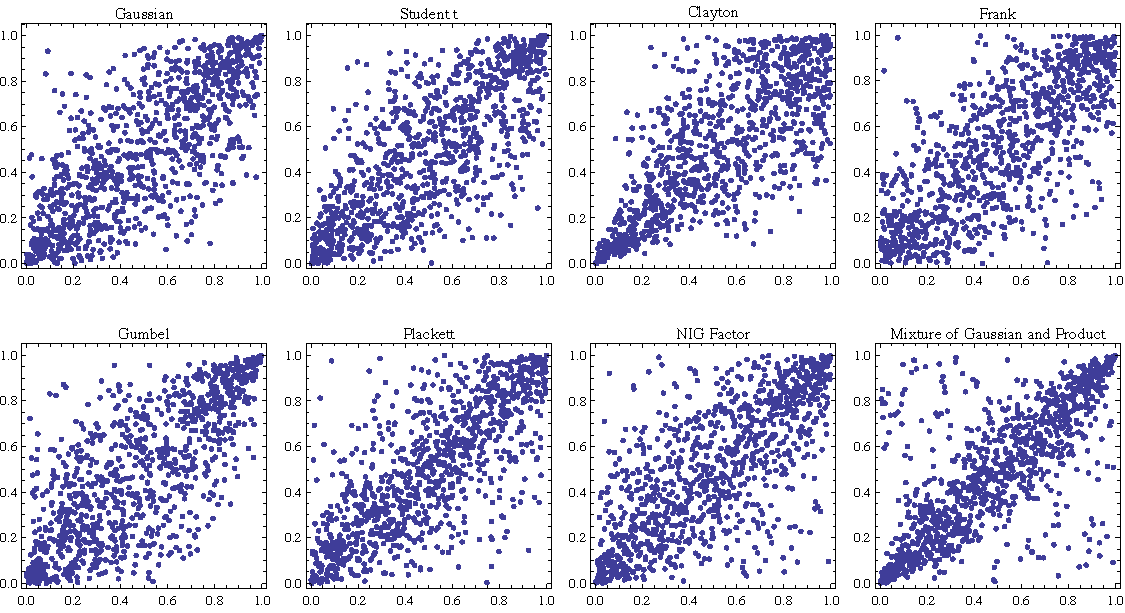
\includegraphics[width=\textwidth]{_pics/copulas_scatterplots.pdf}
  \caption{Scatterplots of samples drawn from various copulae. All
    copulae are calibrated to Spearman's $\rho$ of 0.75 before
    sampling.}\label{fig:copulaeScatterPlot} 
\end{figure}

As this hedging backtest concerns only portfolios with two assets, we
focus on the bivariate version of each copula. 

\subsubsection{Gaussian and $t$ Copulae}\label{sec:ellpitical-copulae}

The Gaussian and $t$ copulae are dervived from Gaussian and $t$
distributions. 

The bivariate Gaussian copula is defined as
\begin{align*}
  \bm{C}(u,v) &= \Phi_{2, \rho}\{\Phi^{(-1)}(u), \Phi^{(-1)}(v)\} \nonumber \\
              &= \int_{-\infty}^{\Phi^{(-1)}(u)}
                \int_{-\infty}^{\Phi^{(-1)}(v)}
                \frac{1}{2\pi\sqrt{1-\rho^2}}
                \exp{\left\{
                \frac{s^2-2\rho st+t^2}{2(1-\rho^2)}
                \right\}} \dd s\, \dd t,\quad, u,v\in [0,1],
\end{align*}
where $\Phi_{2, \rho}$ is the bivariate Normal cdf
with zero mean, unit variance, and correlation coefficient $\rho$, and
$\Phi^{(-1)}$ is the quantile function of the univariate standard normal
distribution.
The Gaussian copula is fully specified by the correlation parameter $\rho$. \footnote{
The symbol $\rho$ is used to denote both the correlation parameter as
well as a general risk measure. However, it will be clear from the
context, what $\rho$ refers to.}
It has no tail dependence, which, in a finance context, implies that
it often underestimates tail risk.  

% The Gaussian copula density is
% \begin{equation*}
%   \bm{c}_\rho(u,v) = \frac{\bm{\varphi}_{2,\rho}\{\Phi^{(-1)}(u), \Phi^{(-1)}(v)\}}
%                      {\varphi\{\Phi^{(-1)}(u)\} \cdot \varphi\{\Phi^{(-1)}(v)\}} 
%                   = \frac{1}{2\pi\sqrt{1-\rho^2}}\exp\left\{
%                      -\frac{u^2 - 2\rho uv + v^2}{2(1-\rho^2)}
%                      \right\},
% \end{equation*}
% where $\bm{\varphi}_{2,\rho}(\cdot)$ is the pdf corresponding to
% $\Phi_{2, \rho}$, and $\varphi(\cdot)$ the standard normal
% pdf. \natp{\em [I think the abbreviations cdf and pdf where not
%   introduced. Please double-check.]}

Kendall's $\tau_K$ and Spearman's $\rho_S$ of the bivariate Gaussian copula are
    \begin{align*}
        \tau_K(\rho) = \frac{2}{\pi}\arcsin\rho
        \end{align*}
    \begin{align*}
        \rho_S(\rho) = \frac{6}{\pi}\arcsin\frac{\rho}{2}.
        \end{align*}

The $t$-copula has the form
\begin{multline*}
        \bm{C}(u,v) = \bm{T}_{2, \rho, \nu}\{T^{(-1)}_\nu(u), T^{(-1)}_\nu(v)\}\\
        = \int_{-\infty}^{T^{(-1)}_\nu(u)}
               \int_{-\infty}^{T^{(-1)}_\nu(v)}
            \frac{\Gamma\left(\frac{\nu+2}{2}\right)}
            {\Gamma\left(\frac{\nu}{2}\right)\pi\nu\sqrt{1-\rho^2}}
             \left(
        1+\frac{s^2-2st\rho+t^2}{\nu}
        \right)^{-\frac{\nu+2}{2}}\, \dd s\, \dd t,
    \end{multline*}
where $\bm{T}_{2, \rho, \nu}$ denotes the 
bivariate $t$ cdf with dependence parameter $\rho$ and degrees of
freedom parameter $\nu$, $\nu>2$,
and where $T^{(-1)}_\nu(\cdot)$ is the quantile function of a standard
$t$ distribution with parameter $\nu$. 

The $t$-copula and Gaussian copula with parameter $\rho$ have equal Kendall's $\tau$, \citep[see][and references therein]{demarta2005t}.

On the other hand, the $t$-copula has a non-zero tail dependence coefficient,
 which makes it more appropriate for dependence modelling in finance. (ref)
% The copula density is
% \begin{align*}
%     \bm{c}(u,v) &= \frac{\bm{t}_{2, \rho, \nu}\{T^{(-1)}_\nu(u), T^{(-1)}_\nu(v)\}}
%     {t_\nu\{T^{(-1)}_\nu(u)\}\cdot t_\nu\{T^{(-1)}_\nu(v)\}},
%     \end{align*}
% where $\bm{t}_{2,\rho, \nu}$ is the pdf of $\bm{T}_{2, \rho, \nu}$
% and $t_\nu$ the density of standard $t$ distribution.

\subsubsection{Archimedean copulae}\label{sec:archimedean-copula}
The family of Archimedean copulae forms a large class of copulae with
many convenient features.
% Contrary to elliptical copulas, which are derived from
% elliptical distributions.
Archimedean copulas are determined via a simple parametric form of the
dependence structure. A prominent feature is the ability to model
asymmetric dependence structures.  

In general, an Archimedean copula takes the form
\begin{align*}
  \bm{C}_\theta(u,v) = \psi^{(-1)}\{\psi(u; \theta), \psi(v; \theta); \theta\},\quad u,v\in [0,1],
    \end{align*}
where $\psi:[0,1] \rightarrow [0,\infty)$ is a continuous, strictly
decreasing and convex function such that $\psi(1)=0$ for any
permissible dependence parameter $\theta$. The function $\psi$ is 
called the generator, with $\psi^{(-1)}$ its inverse.

The {\em Frank copula\/} (B3 in \citet{joe1997multivariate}) takes the form
\begin{align*}
    \bm{C}_{\theta}(u,v) &= \frac{1}{\theta}
    \log \left\{
    1 + \frac{(e^{-\theta u}-1)(e^{-\theta v}-1)}{e^{-\theta}-1}
    \right\}, \quad u,v\in [0,1],
    \end{align*}
    with $\theta \in [0, \infty]$ the dependence parameter. 
    It is a symmetric copula and cannot produce any tail
    dependence. The following parameters correspond perfect dependence
    and independence: $\bm{C}_{-\infty} = \bm{M}$, $\bm{C}_1 = \bm{\Pi}$,
    and $\bm{C}_\infty = \bm{W}$. 
    % The copula density is
    % \begin{align*}
    %   \bm{c}_{\theta}(u,v)
    %   &= \frac{\theta e^{\theta(u+v)(e^\theta-1)}}
    %     {\left\{e^\theta-e^{\theta u}-e^{\theta v}+e^{\theta (u+v)}\right\}^2}.
    % \end{align*}
    The Frank copula has Kendall's $\tau$ :
\begin{align*}
    \tau_K(\theta) = 1-4\frac{D_1\{-\log(\theta)\}}{\log(\theta)},
    \end{align*}
% and
% \begin{align*}
%     \rho_S(\theta) = 1-12\frac{D_2\{-\log(\theta)\} - D_1\{\log(\theta)\}}{\log(\theta)},
%     \end{align*}
where $D_1$ and $D_2$ are the Debye function of order 1 and 2, with
the Debye function defined as $D_n =
\frac{n}{x^n}\int_0^x\frac{t^n}{e^t-1}dt$.
We refer readers to \cite{abramowitz1972handbook}[p.998] for definition of the Debye function. 

The {\em Gumbel copula\/} (B6 in \citet{joe1997multivariate}) has
distribution function
\begin{equation*}
  \bm{C}_{\theta}(u,v) = \exp{-\{ (-\log(u))^\theta +(-\log(v))^\theta 
    \}^{\frac{1}{\theta}}},
\end{equation*}
where $\theta \in [1,\infty)$ is the dependence parameter.
Its  Kendall's tau takes the form \begin{equation*}
  \tau_K(\theta) =\frac{\theta-1}{\theta}. 
 \end{equation*}
It has upper tail dependence with dependence parameter $\lambda^U
= 2-2^{\frac{1}{\theta}}$ and displays no lower tail dependence. 
    
While the Gumbel copula cannot model perfect counter-dependence
\citep{Nelsen2002}, $\bm{C}_{1} = \bm{\Pi}$ models independence, 
and $\lim_{\theta\rightarrow\infty} \bm{C}_\theta = \bm{W}$ models
perfect dependence. 


The {\em Clayton copula\/} takes the form
\begin{equation*}
  \bm{C}_{\theta}(u,v) = \left\{
    \max(u^{-\theta}+v^{-\theta}-1,0)\right\}^{-\frac{1}{\theta}},
\end{equation*}
where $\theta \in (-\infty, \infty)$ is the dependence parameter.
The Clayton copula, by contrast to Gumbel copula,
generates lower tail dependence with $\lambda^L =
2^{-\frac{1}{\theta}}$, but cannot generate upper tail dependence.
Moreover, $\lim_{\theta\rightarrow -\infty} \bm{C}_\theta = \bm{M}$, $\bm{C}_0 =
\bm{\Pi}$, and $\lim_{\theta\rightarrow\infty} \bm{C}_\theta = \bm{W}$. 
Kendall's $\tau$ of the Clayton copula is given by 
\begin{align*}
    \tau_K(\theta) =\frac{\theta}{\theta+2}.
    \end{align*}

\subsubsection{Mixture Copula}\label{sec:mixture-copula}
The mixture copula is a linear combination of copulae. 
The distribution of a 2-dimensional random variable
$\bm{X}=(X_1,X_2)^\top$ is written as linear combination of $K$
copulae 
\begin{equation*} 
    \bm{C}(u,v)= \sum_{k=1}^K p^{(k)} \cdot \bm{C}^{(k)}\{F^{(-1)}_{X_1}(u),
    F^{(-1)}_{X_2}(v); \bm{\theta^{(k)}}\}, \quad u,v\in [0,1].
  \end{equation*}
  Here, $\bm{\theta^{(k)}}$ refers to the parameters of the
    $k$-th copula.
%     Likewise, the copula density is a linear
%     combination of copula densities 
% \begin{align*}
%     \bm{c}(u,v)= \sum_{k=1}^K p^{(k)} \cdot \bm{c}^{(k)}\{F^{(-1)}_{X_1}(u),
%     F^{(-1)}_{X_2}(v); \bm{\theta^{(k)}}\}.
%     \end{align*}
   
While Kendall's $\tau$ of the mixture copula is not known in closed form,
Spearman's $\rho$ is easily derived as 
\begin{equation*}
  \rho_S = \sum_{k=1}^K p^{(k)} \cdot \rho_S^{(k)}. 
\end{equation*}

% \natp{\em [Old text below.]}

% While Kendall's $\tau$ of the mixture copula is not known in closed form,
% Spearman's $\rho$ is specified by the following statement. 
% \begin{proposition}
%   Let $\rho_S^{(k)}$ be Spearman's $\rho$ of the $k$-th component
%   Spearman's $\rho$ of the mixture copula is given by 
%   \begin{align*}
%         \rho_S = \sum_{k=1}^K p^{(k)} \cdot \rho_S^{(k)}.
%         \end{align*}
%     \end{proposition}

% \begin{proof}
%   Since Spearman's $\rho$ is defined as \citep{Nelsen1999}
%   \begin{equation*}
%     \rho_S = 12 \int_{\mathbb{I}^2} \bm{C}(s,t) ds dt - 3,
%   \end{equation*}
%   Spearman's $\rho$ of the the mixture copula is given by summation
%   of the components 
%   \begin{align*}
%     \rho_S = 12 \int_{\mathbb{I}^2} \sum_{k=1}^K p^{(k)} \cdot
%     \bm{C}^{(k)}(s,t) ds dt - 3. 
%   \end{align*}
% \end{proof}
% \natp{\em [Continue here.]}

An example of a mixture copula is the Fr\'echet class of copulae, which
are given by convex combinations of $\bm{W}$, $\bm{\Pi}$, and $\bm{M}$
\citep{Nelsen1999}.  

We use a mixture of Gaussian and independence copulae in our analysis,
i.e., 
\begin{equation*}
  \bm{C}(u,v) = p\, \bm{C}^\text{Gaussian}(u,v) + (1-p)(uv),\quad p\in (0,1).
\end{equation*}
% with corresponding density 
% \begin{equation*}
%   \bm{c}(u,v) = p\, \bm{c}^\text{Gaussian}(u,v) + (1-p).
% \end{equation*}

This mixture models the amount of ``random noise'' that appears in the
off-diagonal region of the dependence structure where the Gaussian copula has no control.
In the hedging exercise, the structure of the off-diagonal ``random noise'' is not our main concern, 
but the amount of it might affect the hedging effectiveness. 

\subsubsection{NIG factor copula}

Normal Inverse Gaussian (NIG) distribution is a flexible and yet analytical tractable distribution introduced by
\citep{BarndorffNielsen1997}.
The {\em NIG factor copula} is constructed based on the characteristics of the NIG disribution. 
We present the reparameterised version of NIG factor copula in this section.

The NIG distribution has density function
\begin{equation*}
  g(x; \alpha,\beta, \mu, \delta) = \frac{\alpha}{\pi} \e^{\delta
    \sqrt{\alpha^2-\beta^2} -\beta\mu} \frac{1}{q((x-\mu)/\delta)}
  K_1\left[\delta \alpha q\left(\frac{x-\mu}{\delta}\right) \right]
  \e^{\beta x},\quad x>0,
\end{equation*}
where $q(x) = \sqrt{1+x^2}$ and where $K_1$ is the modified Bessel
function of third order and index $1$. The parameters satisfy $0\leq
|\beta|\leq \alpha$, $\mu\in \R$ and $\delta>0$. The parameters have
the following interpretation: $\mu$ and $\delta$ are location and
scale parameters, respectively, $\alpha$ determines the heaviness of
the tails and $\beta$ determines the degree of asymmetry. If
$\beta=0$, then the distribution is symmetric around $\mu$.

The cdf and quantile function of NIG distribution, denoted by $G(x; \alpha, \beta, \mu, \delta)$ and $G^{(-1)}(x; \alpha, \beta, \mu, \delta)$,
 have no known analytical form.
 In this work, they are computed via numerical integration of the density and by simulation.

The NIG distribution belongs to
the class of so-called {\em normal
variance-mean mixture distributions},  (see Section 3.2 of 
\citep{McNeil2005}): $X$ follows an
$\text{NIG}(\alpha,\beta,\mu,\delta)$ distribution if $X$ conditional
on $W$ follows a normal distribution with mean $\mu+\beta W$ and
variance $W$, i.e., 
\begin{equation*}
  X|W\stackrel{\mathcal L}\sim \Ncdf(\mu + \beta W, W),
\end{equation*}
where $W$ follows an {\em inverse Gaussian distribution}, denoted by
$\text{IG}(\delta, \sqrt{\alpha^2-\beta^2})$.

Simulation procedure of NIG$(\alpha, \beta, \mu, \delta)$ distribution is a natural result of the above decomposition. 
To simulate the NIG distribution, first simulate a random variable $w \sim IG(\delta, \sqrt{\alpha^2-\beta^2})$, 
then simluate $x \sim N(\mu+ \beta w, w)$ given $w$.

The moment-generating function of the NIG distribution is given by
\begin{equation*}
  M(u; \alpha, \beta, \mu, \delta) = \exp\left( \delta
    \left(\sqrt{\alpha^2-\beta^2} - \sqrt{\alpha^2 - (\beta +
        u)^2}\right) + \mu u\right). 
\end{equation*}
As a direct consequence, moments are easily calculated with the
expectation and variance of the NIG distribution being
\begin{align*}
  \mathbb E X &= \mu +
                \frac{\delta \beta}{\sqrt{\alpha^2-\beta^2}}
  \end{align*}
\begin{align} \label{eq:5}
  \text{Var}(X) &= \frac{\alpha^2\delta}{(\alpha^2-\beta^2)^{3/2}}.
\end{align}

It is easily seen from the moment-generating function that the NIG distribution is preserved under linear combinations, provided
the variables share the parameters $\alpha$ and $\beta$. 
\begin{proposition}
  \label{prop:NIG}
  Let $Z\sim \text{NIG}(\alpha, \beta, \mu, \delta)$ and
  $Z_i\sim \text{NIG}(\alpha, \beta, \mu_i, \delta_i)$,
  $i=1,\ldots, n$ be independent NIG-distributed random
  variables. Then:
  \begin{enumerate}
  \item  $X_i = Z + Z_i\sim \text{NIG}(\alpha,\beta,\mu+\mu_i,
  \delta+\delta_i)$,
\item and 
  \begin{align}
    \text{Cov}(X_i,X_j) &= \text{Var(Z)},\nonumber\\
    \text{Corr}(X_i,X_j) &= \frac{\delta}{\sqrt{(\delta+\delta_i)
                           (\delta+\delta_j)}}. \label{eq:6}
  \end{align}
\end{enumerate}
\end{proposition}
\begin{proof}
  \begin{enumerate}
  \item This follows directly from the moment-generating function. 
  \item For the covariance,
    \begin{equation*}
      \text{Cov}(X_i,X_j)
      = \E[(Z+Z_i) (Z+Z_j)] - \E[Z+Z_i] \E[Z+Z_j]
      = \E[Z^2] -(\E Z)^2.
    \end{equation*}
    The correlation is determined directly from \ref{eq:5}.
  \end{enumerate}
\end{proof}

The NIG distribution is popular in many areas of
financial modelling; for example, it gives rise 
to the normal inverse Gaussian L\'evy process, which may be represented
as a Brownian motion with a time change.
In the setting here, we consider the {\em NIG factor copula}, which is
not directly derived from the multivariate NIG distribution, but
determined through a factor structure instead. \footnote{The factor structure,
which was applied e.g.\ in \citep{Kalemanova2007} for calibrating CDO's,
gives additionaly flexibility as it does not force the components to
have a mixing variable $W$.}

Denote 
\begin{align*}
  X &= Z + Z_1 \\ 
  Y &= Z + Z_2,
  \end{align*}
where $Z \sim \text{NIG}(\alpha, \beta, \mu, \delta)$, $Z_1 \sim \text{NIG}(\alpha, \beta, \mu_1, \delta_1)$, 
$Z_2 \sim \text{NIG}(\alpha, \beta, \mu_2, \delta_2)$, and $Z, Z_1, Z_2$ are mutually independent. 

The following reparameterisation steps reduce the number of parameters to three:
\begin{enumerate}
  \item Set $\mu = \mu_1= \mu_2 = 0$ . Location parameter does not affect the correlation structure.
  \item Set $\delta = \frac{(\alpha^2-\beta^2)^{3/2}}{\alpha^2}$, $\delta_1 = \delta_2$, $\tilde \delta = \delta_1 = \delta_2$. 
  The dependence between X and Y is fully captured by $\alpha, \beta$, and $\tilde \delta$.  
\end{enumerate}
  % Denote the margins by $u,v \sim U(0,1)$. 
% The NIG factor model is obtained by transforming the unifrom margins to standardised NIG distriutions.

\begin{prop}
  Let $u,v \in [0,1]$, $f(\cdot) = g\left(\cdot; \alpha, \beta, 0, \frac{(\alpha^2-\beta^2)^{3/2}}{\alpha^2}
  \right)$, and $F (\cdot) = G(\cdot; \alpha, \beta, 0, \tilde \delta)$, 
  the {\em NIG factor copula} is 
  \begin{equation*}
    C(u,v) = \int_\mathbb{R} F(u-z)F(v-z)f(z)dz,
  \end{equation*}
  where $\alpha, \beta \in \mathbb{R}$ satisfying $0 \leq |\beta| \leq \alpha$, and $\tilde \delta >0 $.
\end{prop}

% The parameters $\alpha, \beta, \tilde \delta$ fully control the dependence between $u$ and $v$, $u, v \sim U(0,1)$, captured by the NIG factor copula.
We refer readers to \cite{krupskii2013factor} for the methodology of constructing a factor copula. 

The quantile dependence and Spearman rho of NIG factor copula have no known analystical form.
In this work, the quantile dependence is computed numerically; 
the Spearman rho is approximated by the Spearman rho of the bivariate Gaussian copula. 
When $\beta \rightarrow 0$ and $\alpha \rightarrow \infty$, the NIG distribution behaves similarly to Gaussian distribution, 
making the NIG factor copula (bivariate) behaves similarly to the Gaussian copula (bivariate). 
Therefore, the NIG factor copula's Spreaman rho is well approximated by the Spearman rho of the bivariate Gaussian copula.


% \natp{\em [Please clarify that $\circ$ refers to composition. Clean
%   up notation, e.g.\ marginals can be denoted $F_F$ and $F_S$, Use
%   just $C$ for the copula. What are $Z_1$ and $Z_2$? I don't find the
%   formula in the paper mentioned. Also, where is the formula for
%   Kendall's tau taken from?]}
%  The NIG factor copula is obtained by transforming the margins to
% uniforms (see Sklar's Theorem), giving (e.g.\
% \citep{krupskii2013factor}):
% \begin{equation*}
%   C_{r^S, r^F}(F_{r^S}(r^S), F_{r^F}(r^F)) = \int_\mathbb{R}
%   F_{Z_1}(F_{X_1}^{(-1)} \circ F_{r^S}(r^S) -z) \cdot
%   F_{Z_2}(F_{X_2}^{(-1)} \circ F_{r^F}(r^F) -z) \cdot
%   f_Z(z) dz.
%   \end{equation*}
% If the margins are continuous, then Spearman's rho of NIG factor
% copula is 
% \begin{equation*}
%   \rho_S = 12 \int \int \int_{\mathbb{R}^3}
%   F_{X_1}(x_1) \cdot
%   F_{X_2}(x_2) \cdot
%   f_{Z_1}(x_1-z) \cdot
%   f_{Z_2}(x_2-z) \cdot
%   f_Z(z) dx_1 dx_2 dz - \frac{1}{48}.x
%   \end{equation*}

% \begin{proof}
%   \begin{align}
%   \rho_S(r^S, r^F) &= \rho\{F_{r^S}(r^S), F_{r^F}(r^F)\} \\
%     &= \rho\{F_{X_1}(X_1), F_{X_2}(X_2)\} \\
%     &= 12 \cdot \mathbb{E}\{F_{X_1}(X_1) \cdot F_{X_2}(X_2) \} - \frac{1}{48}\\
%     &= 12 \cdot \int \int_{\mathbb{R}^2} F_{X_1}(X_1) \cdot F_{X_2}(X_2) dF_{X_1,X_2}(x_1,x_2)\\
%     \end{align}
%   Because
%   \begin{align}
%     F_{X_1,X_2}(x_1,x_2) &= \mathbb{P}(X_1 \leq x_1, X_2 \leq x_2)\\
%     &= \mathbb{P}(Z_1 \leq x_1 - Z, Z_2 \leq x_2 - Z) \\
%     &= \int_\mathbb{R}\mathbb{P}(Z_1 \leq x_1 - z) \cdot \mathbb{P}(Z_2 \leq x_2 - z) \cdot f_Z(z) dz,
%     \end{align}
%   so,
%   \begin{align}
%     \rho_S(r^S, r^F) = 12 \cdot \int \int \int_{\mathbb{R}^3} F_{X_1}(x_1) \cdot F_{X_2}(x_2) \cdot f_{Z_1}(x_1 -z) \cdot f_{Z_2}(x_2 -z) \cdot f_{Z}(z) dx_1 dx_2 dz -\frac{1}{48}
%     \end{align}
%   \end{proof}


\subsubsection{Plackett copula}\label{subsec:other-copula}
The Plackett copula has distribution function
\begin{align*}
    \bm{C}_{\theta}(u,v) &= \frac{1+(\theta-1)(u+v)}{2(\theta-1)}
                         - \frac{\sqrt{\{
    1+(\theta-1)(u+v)\}^2 - 4uv\theta(\theta-1)}}{2(\theta-1)},
\end{align*} where $0 \leq \theta < \infty$.
Spearman's Rho is given by 
\begin{align*}
    \rho_S(\theta) = \frac{\theta+1}{\theta-1} - \frac{2\theta \log
  \theta}{(\theta-1)^2}. 
    \end{align*}

The Placket copula possesses a special property:
the cross-product ratio is equal to the dependence parameter
\begin{equation} \label{eq:PlackettCrossProduct}
    % &\phantom{=}
    \frac{\p(U \leq u, V \leq v) \cdot \p(U > u, V > v)}
    {\p(U \leq u, V > v) \cdot \p(U > u, V \leq v)}\nonumber
    =
      \frac{\bm{C}_\theta(u,v)\{1-u-v+\bm{C}_\theta(u,v)\}}{\{u-\bm{C}_\theta(u,v)\}\{v-\bm{C}_\theta(u,v)}\nonumber 
    = \theta.
\end{equation}
In words, the dependence parameter is equal to the ratio of the 
number of concordance pairs and the number of discordance pairs of a 
bivariate random variable. 

%! Author = francis
%! Date = 30.10.20

\subsection{Calibration and selection of copulae}\label{sec:estimation}
We introduce the method to calibrate copulae to our data in this section.
In general, there are two types of calibration procedures to calibrate copulae:
maximum likelihood (MLE) and method of moments (MM).
We decide to deploy the latter since it calibrates according to the moments we desired. \medskip

In the following subsection, we present the configuration of the method of moments procedures we use.
In the subsection after, we argue that MM is more suitable to this work by comparing MM with MLE.

\subsubsection{Method of Moments}
\label{subsec:simulated-method-of-moments}

We trace back the usage of MM to calibrate copulae to \citet{Genest1987, genest1993statistical}.
The moments mainly refer to Kendall's $\tau$ or Spearman's $\rho$.
We extend MM to quantile dependence measures denoted by $\lambda_q$ for quantile level $q$.

Spearman's $\rho$, Kendall's $\tau$, and quantile dependence of the copula $C$ are defined as
\begin{align}
  \rho_S &= 12 \int\int_{I^2} C_{\bm{\theta}}(u,v)\, \dd u\, \dd v-3\label{eq:rho_S}\\
  \tau_K &= 4\E[C_{\bm{\theta}}\{F_X(x), F_Y(y)\}]-1,\\
  \lambda_q &=
  \begin{cases}
    \p(F_X(X)\leq q| F_Y(Y)\leq q) = \displaystyle \frac{C_{\bm{\theta}}(q,q)}{q},
    &\text{ if } q\in (0,0.5],\\
    \p(F_X(X)>q|F_Y(Y)>q) =\displaystyle \frac{1-2q+C_{\bm{\theta}}(q,q)} {1-q},
    &\text{ if } q\in (0.5,1).
  \end{cases}
\end{align}\medskip
The empirical counterparts are
\begin{align*}
  \hat\rho_S &= \frac{12}{n} \sum_{k=1}^n \hat F_X(x_k) \hat F_Y(y_k)
               -3,\\
  \hat\tau_K &= \frac{4}{n}\sum_{k=1}^n \hat{C}\{\hat{F}_X(x_i),\hat{F}_X(y_i)\} -1 ,\\
  \hat\lambda_q &=
                  \begin{cases}
                    \displaystyle\frac{1}{n} \sum_{k=1}^n \frac{\1_{\{\hat
                        F_X(x_k)\leq q, \hat F_Y(y_k)\leq q\}}} {q},
                    &\text { if } q\in (0, 0.5],\\
                    \displaystyle \frac{1}{n} \sum_{k=1}^n
                    \frac{\1_{\{\hat F_X(x_k)>q, \hat F_Y(y_k)>q\}}}
                    {1-q}, &\text { if } q\in (0.5,1),
                  \end{cases}
\end{align*}
where $\displaystyle \hat{F}(x) =
  \frac{1}{n}\sum_{k=1}^n 1_{\{x_i\leq x\}}$ and
$\displaystyle \hat{C}(u,v) = \frac{1}{n}\sum_{k=1}^n 1_{\{u_i\leq u, v_i\leq v\}}$. \medskip

Denote by $\bm{m}(\bm{\theta})$ the $m$-dimensional vector of
dependence measures according the dependence parameters
$\bm{\theta}$,and let $\hat{\bm{m}}$ be the corresponding empirical
counterpart. 
The difference between dependence measures and their counterpart is denoted by
\begin{align*}
    \bm{g}(\bm{\theta}) = \hat{\bm{m}} - \bm{m}(\bm{\theta}).
\end{align*}

The MM estimator is
\begin{align*}
    \hat{\bm{\theta}} = \argmin_{\bm{\theta}\in \bm{\Theta}} \bm{g}(\bm{\theta})^\top
    \hat{\bm{W}}
     \bm{g}(\bm{\theta}),
\end{align*}
where $\hat{W}$ is some positive definite weight matrix.
In this work, we use
$\bm{m}(\bm{\theta}) = (\rho_S, \lambda_{0.05}, \lambda_{0.1}, 
\lambda_{0.9}, \lambda_{0.95})^\top$
for calibration.
$\hat{W}$ is set to identity matrix.

\subsubsection{Comparison of method of moments and maximum likelihood}
\label{subsec:maximum-likelihood-estimation}
By the Hoeffding-Sklar theorem, the joint density of a $d$-dimensional random variable $\bm{X}$ with sample size $n$ can be written as
\begin{equation*}
    \bm{f}_{\bm{X}}(x_1, ..., x_d) = \bm{c}\{F_{X_1}(x_1), ..., F_{X_d}(x_d)\} \prod_{j=1}^d f_{X_i}(x_i).
    \end{equation*}
We follow the treatment of MLE documented in section 10.1 of
\citet{joe1997multivariate}, namely the {\em inference functions for
margins (IFM) method}.
The log-likelihood $\sum^n_{i=1}f_{\bm{X}}(X_{i,1}, ..., X_{i,d})$ can be decomposed into a dependence part and a marginal part,
\begin{align}
    L(\bm{\theta}) &= \sum_{i=1}^n \bm{c}\{F_{X_1}(x_{i,1};\bm{\delta}_1), ..., F_{X_d}(x_{i,d}; \bm{\delta}_d);\bm{\gamma}\}
    + \sum_{i=1}^n \sum_{j=1}^d f_{X_j}(x_{i,j};\bm{\delta}_j)\\
    &= L_C(\bm{\delta}_1, ..., \bm{\delta}_d, \bm{\gamma}) + \sum_{j=1}^d L_j(\bm{\delta}_j)
    \end{align}
where $\bm{\delta}_j$ are the parameters of the $j$-th margin, $\bm{\gamma}$ is the parameter of the parametric copula, and
$\bm{\theta} = (\bm{\delta}_1,..., \bm{\delta}_d, \bm{\gamma})$.
Instead of searching the $\bm{\theta}$ in a high dimensional space, \citet{joe1997multivariate} suggests to
search for $\hat{\bm{\delta}_1},..., \hat{\bm{\delta}_d}$ that maximize $L_1(\bm{\delta}_1), ..., L_d(\bm{\delta}_d)$,
then search for $\hat{\bm{\gamma}}$ that maximize $L_C(\hat{\bm{\delta}_1},..., \hat{\bm{\delta}_d}, \bm{\gamma})$.

%\natp{\em [I suggest to delete the next part, as the regularity
%  conditions are unclear, and it is just a first-order condition,
%  which is a-priori not clear to hold in a two-step procedure.]}
%That is, under regularity conditions, $(\hat{\bm{\delta}_1},..., \hat{\bm{\delta}_d}, \hat{\bm{\gamma}})$ is the solution of
%\begin{align}
%    \left( \frac{\partial L_1}{\partial \bm{\delta}_1}, ..., \frac{\partial L_d}{\partial \bm{\delta}_d},
%    \frac{\partial L_C}{\partial \bm{\gamma}}\right) = \bm{0}.
%    \end{align}

%However, the IFM requires making assumption on the distribution of the
%margins.\natp{\em [delete until here.]}

We follow \citet{genest1995semiparametric} who suggest to replace the estimation of marginals parameters estimation by non-parameteric estimation.
Given non-parametric estimator $\hat{F}_i$ of the margins $F_i$, the estimator of the dependence parameters $\bm{\gamma}$ is
\begin{equation*}
    \hat{\bm{\gamma}} = \argmax_{\bm{\gamma}} \sum_{i=1}^n \bm{c}\{ \hat{F}_{X_1}(x_{i,1}), ..., \hat{F}_{X_d}(x_{i,d});\bm{\gamma}\}.
    \end{equation*}

Both the simulated method of moments and the maximum likelihood estimation are unbiased.
The question though which procedure is more suitable for hedging.

\begin{figure}[h]
%\includegraphics[width=\textwidth]{_pics/t Copula quantile dependence.png}
\includegraphics[width=\textwidth]{_pics/Gumbel Copula quantile dependence.pdf}
\includegraphics[width=\textwidth]{_pics/Clayton Copula quantile dependence.pdf}
  \caption{Quantile dependences of Gumbel, and Clayton Copula. The \textcolor{darkblue}{blue circle dots} are
  the quantile dependence estimates of Bitcoin and CME future, \textcolor{darkblue}{blue dotted lines} are the estimates' 90\% confidence interval.
  \textcolor{orange}{Orange dotted line} is the copula implied quantile dependence by MM estimation.
  \textcolor{lightblue}{Light blue dotted line} is the copula implied quantile dependence by MLE estimation.
%  \href{http://www.quantlet.com/}{\includegraphics[height=\baselineskip]{_pics/qletlogo_tr.png}}
  }
\label{fig:quantile dependence1}
\end{figure}

Figure~\ref{fig:quantile dependence1} shows the empirical quantile dependence of Bitcoin and CME future and the copula implied
quantile dependence of the MLE and MM calibration procedures.
Although the MLE is a better fit to a range of quantile dependence in the middle, it fails to address the situation in the tails.
We find that our data empirically has low quantile dependence in the lower ends ($q<10\%$).
We argue that MM is preferred as it produces a better fit to the dependence
structure in the tail behaviour, contrary to MLE. \medskip

Therefore, we deploy the method of moments throughout the
analysis.
We choose the $5^\text{th}$-, $10^\text{th}$-, $90^\text{th}$-, $95^\text{th}$-quantile, and Spearman's $\rho$ as the moments.


%
%
%\subsection{Two-Stage Estimation}\label{subsec:two-stage-estimation}
%~\cite{joe2005asymptotic} study the efficiency of a two-stage estimation procedure of copula estimation.
%The authors also call this method inference function for margins IFM.
%
%\textbf{Pros}
%\begin{enumerate}
%    \item Almost as efficient as MLE methods but easier to be implemented
%    \item Yields an asymptotically Gaussian, unbiased estimate
%\end{enumerate}
%
%\textbf{Cons}
%\begin{enumerate}
%    \item Subject to specification of marginals \cite{kim2007comparison}
%\end{enumerate}
%
%Our data
%\begin{align}
%    \pmb{y} = \begin{bmatrix}
%                  y_{11} & \cdots & y_{1i}\\
%                  \vdots & \ddots & \vdots \\
%                  y_{n1} & \cdots & y_{ni}
%                  \end{bmatrix}
%    \end{align}
%Let $F$ and $f$ be the joint cdf and joint density of $\pmb{y}$ with parameters $\pmb{\delta}$,
%and let $F_i$ and $f_i$ be the marginal cdf and marginal density for the $i^\text{th}$ random variable with parameters $\pmb{\theta}_i$, we have
%\begin{align}
%    f(\pmb{y}; \pmb{\theta}_1, \pmb{\theta}_2,\dots \pmb{\theta}_i, \pmb{\delta}) =
%    c\{F_1(\pmb{y}_1;\pmb{\theta}_1), F_2(\pmb{y}_2; \pmb{\theta}_2), \dots, F_i(\pmb{y}_1;\pmb{\theta}_i); \pmb{\delta}\}
%    \prod^i_{j=1}f_i(\pmb{y}_j;\pmb{\theta}_j)
%    \end{align}
%
%For a sample of size $n$, the log-likelihood of functions of the $i^\text{th}$ univariate margin is
%\begin{align}
%    L_i(\theta_i) = \sum^n_{m=1} \log f_i(y_{mi}; \theta_i),
%    \end{align}
%
%and the log-likelihood function for the joint distribution is
%\begin{align}
%    L(\delta, \theta_1, \theta_2, \dots, \theta_i) = \sum^n_{m=1}\sum^i_{j=1} \log f(y_{mj}; \delta, \theta_1, \theta_2, ..., \theta_i)
%    \end{align}
%
%In most cases, one does not have closed form estimators and numerical techniques are needed.
%Numerical ML estimation difficulty increase when the total number of parameters increases.
%The two-stage estimation is designed to overcome this problem.
%
%The two-stage procedure is
%\begin{enumerate}
%    \item estimate the univariate parameters from separate univariate likelihoods to get $\tilde{\pmb{\theta}_1}, ..., \tilde{\pmb{\theta}_i}$
%    \item maximize $L(\pmb{\delta}, \tilde{\pmb{\theta}_1}, \dots, \tilde{\pmb{\theta}_i})$ over $\pmb{\delta}$ to get $\tilde{\pmb{\delta}}$
%    \end{enumerate}
%
%Under regularity conditions
%\footnote{Regularity conditions include
%1. $\exists \frac{\partial \log f(x;\theta)}{\partial \theta}, \frac{\partial^2 \log f(x;\theta)}{\partial \theta^2}, \frac{\partial^3 \log f(x;\theta)}{\partial \theta^3}$ for all $x$;
%2. $\exists g(x), h(x) and H(x)$ such that for $\theta$ in a neighborhood $N(\theta_0)$ the relations
%$\left|\frac{\partial f(x;\theta)}{\partial theta}\right| \leq g(x)$,
%$\left|\frac{\partial^2 f(x;\theta)}{\partial \theta^2}\right| \leq h(x)$,
%$\left|\frac{\partial^3 f(x;\theta)}{\partial \theta^3}\right| \leq H(x)$ hold for all $x$, and
%$\int g(x) dx < \infty$, $\int h(x) dx < \infty$, $\mathbb{E}_\theta \{H(X)\} < \infty$ for $\theta \in N(\theta_0)$;
%3. For each $\theta \in \Theta$, $0< \mathbb{E}_\theta \left\{
%\left(
%\frac{\partial \log f(X;\theta)}{\partial \theta}
%\right)^2
%\right\}$. For detail see section 4.2.2 of~\cite{serfling2009approximation}}
%, $(\pmb{\tilde{\theta}}_1,\dots \pmb{\tilde{\theta}}_i, \pmb{\tilde{\delta}})$ is the solution of
%\begin{align}
%    (\partial L_1 / \partial \pmb{\theta}^\intercal_1,
%    \dots, \partial L_i / \partial \pmb{\theta}^\intercal_i, \partial L / \partial \pmb{\pmb{\delta}}^\intercal_1) = \pmb{0}
%    \end{align}
%
%For comparison, if we optimize $L$ directly without the two-stage procedure (i.e.~MLE), we solve for
%\begin{align}
%    (\partial L / \partial \pmb{\theta}^\intercal_1,
%    \dots, \partial L / \partial \pmb{\theta}^\intercal_i, \partial L / \partial \pmb{\pmb{\delta}}^\intercal_1) = \pmb{0}
%    \end{align}
%
%We denote the two solutions as
%$\tilde{\pmb{\eta}} = (\pmb{\tilde{\theta}}_1,\dots \pmb{\tilde{\theta}}_i, \pmb{\tilde{\delta}})$ for two-stage procedure;
%$\hat{\pmb{\eta}} =(\pmb{\hat{\theta}}_1,\dots \pmb{\hat{\theta}}_i, \pmb{\hat{\delta}})$ for MLE procedure.
%and compare the asymptotic relative efficiency of $\tilde{\pmb{\eta}}$ and $\hat{\pmb{\eta}}$.
%
%Asymptotics: yet to be done.\\
%~\cite{kim2007comparison} show the estimation of $\pmb{\theta}$ may be seriously affected.
%They compare the two-stage approach and Canonical Maximum Likelihood Method by simulation and
%conclude that Canonical Maximum Likelihood is prefered from a computational statistics and data analysis point of view.
%
%\subsection{Canonical Maximum Likelihood Method}\label{subsec:canonical-maximum-likelihood-method}
%This approach was studied by~\cite{genest1995semiparametric} and~\cite{shih1995inferences}.
%One estimates the margins using empirical CDF
%\begin{align}F_X(x)=\frac{1}{n+1}\sum_{i=1}^n 1(X_i \leq x)\end{align},
%
%we maximize the log-likelihood
%\begin{align}
%    L(\delta) = \sum_{i=1}^n \log [c_\delta \{F_X(X_i), F_Y(Y_i)\}]
%    \end{align}
%
%This procedure does not require specification of marginals.
%
%
%
%
%
%%also by Wang and Ding, 2000; Tsukahara, 2005
%%This is also known as pseudo maximum likelihood (PML) and as canonical maximum likelihood (see Cherubini et al., 2004)
%%
%%Genest and Werker (2002) obtained conditions under which the PMLE is asymptotically efficient.
%%
%%


%%% Local Variables:
%%% mode: latex
%%% TeX-master: "SRM"
%%% End:

% ----------------
% --- Estimation of Copula ---
% ----------------

\subsubsection{Copula selection}\label{subsec:copula-selection}
As the dependence structure of price data changes
across time, we allow for a flexible choice of the best-fitting
copula, by re-calibrating periodically and re-evaluating performance
of the various copulas. 
In each re-calibration, we select the best-fitting
copula, characterised by the lowest {\em Akaike Information Criterion
  (AIC)},
\begin{equation*}
 \text{AIC} = 2k- 2 \log(L),
\end{equation*}
where $k$ is the number of estimated
parameteres and $L$ is the likelihood \citep{Akaike1973}. 

% they tend to suggest the same copula as the best fitting one.
%Simulation studies has also been carried out to compare different copula selection methods, see \cite{}.
Other model selection criteria, such as the TIC~\citep{takeuchi1976distribution} or likelihood ratio test could be used instead.
For a survey of model selection and inference, see \cite{anderson1998comparison}.
Among various copula selection procedures, AIC is a popular choice for
its applicability, see e.g. \cite{breymann2003dependence}.
In our case, the AICs are calculated only with dependence likelihood
since the marginals are modelled via kernel density estimators.
The selected copula will then enter the calculation of the optimal
hedge ratio.
% We consider the copula with the lowest AIC for a particular set of data the best fitting one and use it to generate OHR.

\subsection{Risk measures}\label{subsec:spectral-risk-measures}
The optimal hedge ratio is determined for the following variety of risk measures: variance, Value-at-Risk (VaR), Expected Shortfall (ES), and Exponential Risk Measure (ERM).
A summary of risk measures being used in portfolio selection problem
can be found in \citet{hardle2008applied}. 
The risk measures here serve as risk minimization objectives, i.e. loss functions for searching the optimal hedge ratio. 
%They are used in many literature about hedging, e.g. ;
%The risk measures are also used by regulatory bodies,
%for example Basel III ....

The risk measures are defined as follows.
Let $Z$ be a random
variable with distribution function $F_Z$.
\begin{enumerate}
\item Variance: $\text{Var}(Z) = \E[(Z-\E Z)^2]$. 
\item VaR at confidence level $\alpha$: $\text{VaR}_\alpha(Z) = -F_{Z}^{(-1)}(1-\alpha)$
\item ES at confidence level $\alpha$: $\text{ES}(F_Z) = -\frac{1}{1-\alpha}\int_0^{1-\alpha}F_Z^{(-1)}(p)dp$
\item ERM with Arrow-Pratt coefficient of absolute risk
  aversion $k$:
  \begin{equation*}
    \text{ERM}_k(F_Z) = \int_0^{1-\alpha}\phi(p) F_Z^{(-1)}(p)dp,
  \end{equation*}
  where $\phi$ is a weight function described in (\ref{eq:phi}) below.
\end{enumerate}

VaR, ES, and ERM fall into the class of spectral risk measures (SRM),
which have the form \citep{Acerbi2002}%, adam2008spectral,dowd2008spectral}
\begin{equation*}
  \rho_\phi(r^h) = - \int_0^1 \phi(p) F_{Z}^{(-1)}(p)d p,
\end{equation*}
where $p$ is the loss quantile and $\phi(p)$ is a user-defined
weighting function defined on $[0,1]$.
We consider only so-called admissible risk spectra $\phi(p)$, i.e.,
fulfilling %(named by \citet{Acerbi2002})
\begin{enumerate}[label=(\roman*)]
\item $\phi$ is positive,
\item $\phi$ is decreasing,
\item and $\int\phi=1$. 
\end{enumerate}

The VaR's $\phi(p)$ gives all its weight on the $1-\alpha$ quantile of
$Z$ and zero elsewhere, i.e., the weighting function is a Dirac delta
function, and hence it violates the (ii) property of admissible risk
spectra.  
The ES' $\phi(p)$ gives all tail quantiles the same weight of
$\displaystyle\frac{1}{1-\alpha}$ and non-tail quantiles zero weight. 
The ERM assumes investors' risk preference are in the form of an
exponential utility function $U(x)=1-e^{kx}$, so its corresponding
risk spectrum is defined as
\begin{equation*}
  \phi(p) =\frac{k e^{-k(1-p)}}{1-e^{-k}} , \label{eq:phi}
\end{equation*}
where $k$ is the Arrow-Pratt coefficient of absolute risk aversion. 
The parameter $k$ has an economic interpretation as being the ratio
between the second derivative and first derivative 
of investor's utility function on an risky asset,
\begin{equation*}
  k = -\frac{U''(x)}{U'(x)},
\end{equation*}
for $x$ in all possible outcomes.
In case of the exponential utility, $k$ is the the constant absolute risk aversion (CARA).


\input{D1Operator.tex}

\section{Special copulas}
\label{sec:dependence}

\natp{Add basics about copulas, Sklar's Theorem}

Currently: Archimedean (Clayton, Gumbel), Gaussian, NVM / elliptical
(Student $t$, NIG), NIG factor

Possibly: double $t$, Frank, skewed-$t$

\natp{For CF-expansion of Student $t$, see Abramowitz Stegun 26.7.5,
  see also \url{https://citeseerx.ist.psu.edu/viewdoc/download?doi=10.1.1.152.7540&rep=rep1&type=pdf}}


\subsection{Gaussian Copula}\label{subsec:Gaussian-copula}

The {\bf Gaussian copula}, also called {\bf Normal
    copula}, is the copula generated by jointly normally
  distributed random variables (given here in bivariate form):
\begin{equation*}
  C_{\rho,\Ncdf}(u,v) := \Ncdf_2(\Ncdf^{(-1)}(u), \Ncdf^{(-1)}(v);
  \rho), 
\end{equation*}
where $\Ncdf_2$ and $\Ncdf$ are the bivariate and univariate normal
distribution functions, respectively, and $\rho $ is the correlation
parameter. 
\begin{figure}[t]
  \centering
  \includegraphics[scale=.35]{_pics/copulas/normal1.pdf}  
  \includegraphics[scale=.35]{_pics/copulas/normal2.pdf}  
  \caption{Left: Density of the Gaussian (Normal) copula. Right:
    pdf of the bivariate Normal distribution ($\rho=0.5$ in both
    cases).} 
  \label{fig:normalcopula}
\end{figure}

The Gaussian or Normal copula is
\begin{align}
    C^{Ga}_\Sigma(x) &= \frac{1}{(2\pi)^{d/2} |\Sigma|^{1/2}}
    \int_{-\infty}^{\Phi^{-1}(x_1)} \dots \int_{-\infty}^{\Phi^{-1}(x_d)}
    \exp \left\{
    -\frac{1}{2}y^\top \Sigma^{-1}y
    \right\}
    dy_1 \dots dy_d, \quad x\in \R^d.
    \end{align}

The copula density is
\begin{align}
    c^{Ga}_\Sigma(x) &= \frac{1}{(2\pi)^{d/2} |\Sigma|^{1/2}}
    \exp \left\{
    -\frac{1}{2}\begin{pmatrix} \Phi^{-1}(x_1) \\ \vdots \\ \Phi^{-1}(x_d) \end{pmatrix}^\top \Sigma^{-1} \begin{pmatrix} \Phi^{-1}(x_1) \\ \vdots \\ \Phi^{-1}(x_d) \end{pmatrix}
    \right\}
    \end{align}

Simplified notation bivariate Gaussian copula
\begin{align}
       C^{Ga}_\rho \{w, g(w)\} &= \Phi_\rho [\Phi^{-1}(w), \Phi^{-1}\{g(w)\}],
\end{align}
where $g(w): [0,1] \mapsto \mathbb{R}$ is defined above,
$\rho$ is the dependency parameter of a bivariate Gaussian copula,
$\Phi_\rho$ is bivariate normal distribution with mean 0 and covariance $\begin{bmatrix}1 & \rho \\ \rho & 1 \end{bmatrix}$,
$\Phi(\cdot)$ is CDF of standard normal,
$\phi(\cdot)$ is PDF of standard normal,
$\Phi^{-1}(\cdot)$ is quantile function of standard normal.

\natp{\em [I suggest to move the part below to the section where the
  formula for $r^h$ is discussed. Also, there is a simpler version
  that requires only univariate function evluations.]}

The bivariate $D_1 C^{Ga}\{w, g(w)\}$ is
\begin{align}
    D_1 C^{Ga}_\rho\{w, g(w)\} = \int_{-\infty}^{\Phi^{-1}\{g(w)\}} \phi_\rho\{
    \Phi^{-1}(w), u \}du \cdot \frac{1}{\phi\{\Phi^{-1}(w)\}}
    \end{align}
\begin{proof}
    \begin{align}
    D_1 C_\rho\{w, g(w)\}
    &= \left. \frac{\partial C_\rho\{w, g(w')\}}{\partial w}\right|_{w'=w}\\
    &= \left. \frac{\partial \Phi_\rho [\Phi^{-1}(w), \Phi^{-1}\{g(w)\}]}{\partial \Phi^{-1}(w)} \frac{\partial \Phi^{-1}(w)}{\partial w}\right|_{w'=w}\\
    &= \frac{1}{2\pi\rho} \int_{-\infty}^{\Phi^{-1}\{g(w)\}} \exp\left\{
        -\frac{1}{2(1-\rho^2)} \Phi^{-1}(w)^2 - 2\rho\Phi^{-1}(w)u + u^2
        \right\}du
        \cdot \frac{1}{\phi\{\Phi^{-1}(w)\}}
        \end{align}
    \end{proof}

% The bivariate Gaussian Copula density~$c^{Ga}\{w, g(w)\}$ is
% \begin{align}
%     c_\rho^{Ga}\{w, g(w)\} &= \frac{\partial D_1C_\rho^{Ga}\{w, g(w)\}}{\partial g(w)}\\
%                            &= \frac{\phi_\rho [\Phi^{-1}(w), \Phi^{-1}\{g(w)\}]}
%                             {\phi\{\Phi^{-1}(w)\}\phi[\Phi^{-1}\{g(w)\}]}
%     \end{align}


    
\subsubsection*{Hedge distribution}
\label{sec:hedge-distribution-gaussian}

Let $r^S\sim \Ncdf(\mu_S, \sigma_S^2)$ and $r^F\sim \Ncdf(\mu_F,
\sigma_F^2)$ and assume further that they are jointly normally
distributed with correlation $\rho$. Then,
\begin{equation*}
  r^h = r^S - h r^F \sim \Ncdf(\mu_S - h \mu_F, \sigma_s^2 + h^2
  \sigma_F^2 - 2\rho h \sigma_S \sigma_F).
\end{equation*}
More generally, if $R^k\sim F^k$, $k\in \{S,F\}$, then the
distribution of $r^h$ can be expressed with univariate
expressions: 
\begin{align*}
  \p(r^S-h r^F\leq x)
  &= 1-\E\left[ \p\left(r^F\leq \frac{r^S-x}{h}\big| r^S\right)\right] \\ %
  &= 1-\E\left[\p \left(\Ncdf^{(-1)}(F_F(r^F)) \leq
    \Ncdf^{(-1)}\left(F_F\left(\frac{r^S-x}{h}\right)\right) \Big|
    r^S\right)\right] \\%
  &= 1-\E\left[ \p\left(\rho \Ncdf^{(-1)}(F_S(r^S)) + \sqrt{1-\rho^2}
    \varepsilon \leq \Ncdf^{(-1)}\left(F_F\left(\frac{r^S-x}{h}\right)\right) \Big|
    r^S\right)\right]\\ %
  &= 1-\E\left[ \Ncdf \left(
    \frac{\Ncdf^{(-1)}\left(F_F\left(\frac{r^S-x}{h}\right)\right) -\rho
    \Ncdf^{(-1)}(F_S(r^S))} { \sqrt{1-\rho^2}}\right)\right]\\
  &= 1-\int_0^1  \Ncdf \left(
    \frac{\Ncdf^{(-1)}\left(F_F\left(\frac{F_S^{(-1)}(u)-x}{h}\right)\right) -\rho
    \Ncdf^{(-1)}(u)} { \sqrt{1-\rho^2}}\right) \,\dd u.
\end{align*}



\subsection{Archimedean Copulae}
\label{sec:archimedean-copulas}

\begin{itemize}
\item A well-studied one-parameter family of copulae are the {\bf
    Archimedean copulas}. 
\item Let $\phi:[0,1]\rightarrow[0,\infty]$ be a
  continuous and strictly decreasing function with $\phi(1)=0$ and
  $\phi(0)\leq\infty$.
\item  We define the {\bf pseudo-inverse} of $\phi$ as 
  \begin{equation*}
    \phi^{(-1)}(t)=
    \begin{cases}
      \phi^{-1}(t), &0\leq t\leq \phi(0),\\
      0, &\phi(0)<t\leq\infty.
    \end{cases}
  \end{equation*}
\item If, in addition, $\phi$ is convex, then the following function
  is a copula: 
  \begin{equation*}
    C(u,v)=\phi^{(-1)}(\phi(u)+\phi(v)).
  \end{equation*}
  \vspace*{-\baselineskip}
\item Such copulas are called {\bf Archimedean copulas}, and the
  function $\phi$ is called an {\bf Archimedean copula generator}. 
\item Examples of Archimedean copulas are the {\bf Gumbel} and the
  {\bf Clayton} copulas:
  \begin{align*}
    C_{\theta,{\rm Gu}}(u,v) &= \exp\left\{-((-\ln u)^\theta + (-\ln
                               v)^\theta)^{1/\theta}\right\},& 1\leq \theta<\infty,\\
    C_{\theta,{\rm Cl}}(u,v)&= (u^{-\theta} + v^{-\theta}
                              -1)^{-1/\theta}, & 0<\theta<\infty. 
  \end{align*}
\item In the case of the Gumbel copula, the independence copula is 
  attained when $\theta=1$ and the comonotonicity copula is attained
  as $\theta\rightarrow\infty$. 
\item Thus, the Gumbel copula interpolates between independence and
  perfect dependence.  
\item In the case of the Clayton copula, the independence copula is
  attained as $\theta\rightarrow 0$, whereas the comonotonicity
  copula is attained as $\theta\rightarrow\infty$. 
\end{itemize}

\subsection{Elliptical Copulas and normal variance mixtures}
\label{subsec:elliptical-copulae}


\providecommand{\bZ}{\ensuremath{\bm{Z}}}
\providecommand{\bU}{\ensuremath{\bm{U}}}
\providecommand{\bu}{\ensuremath{\bm{u}}}

See e.g.\ Theorem 3.22, Definition 3.26 and Theorem 3.28 of
\citep{McNeil2005}:
\begin{definition}
  A random vector $\bZ=(Z_0,\ldots, Z_d)^T$ follows an elliptical
  distribution if it has a representation
  \begin{equation*}
    \bZ\stackrel{\mathcal L}= G A \bU,
  \end{equation*}
  where $G>0$ is a scalar random variable, the so-called {\em mixing
  variable}, $A$ is a deterministic $(d+1)\times (d+1)$ matrix with
$A A^T:=\Sigma$, which in turn is a $(d+1)\times (d+1)$ nonnegative
definite symmetric matrix of rank $d+1$, and $\bU$ is a
$(d+1)$-dimensional random vector uniformly distributed on the unit
sphere $\mathcal S_{d+1}:=\{\bm{z}\in \R^{d+1}: \bm z^T \bm z=1\}$,
and $\bU$ is independent of $G$.
\end{definition}

A subclass of elliptical distributions are the so-called {\em normal
  variance mixtures (NVM)}, see Section 3.3 of \citep{McNeil2005}. For the
connection between NVM and elliptical distributions, see also Theorem
3.25 of \citep{McNeil2005}. 

\begin{definition}[Normal variance mixture (NVM)]
  The random vector $\mathbf X=(X_1, \ldots, X_k)^T$ follows a
  multivariate {\em normal variance mixture (NVM) distribution} if
  \begin{equation*}
    \mathbf X \stackrel{\mathcal L}{=} \mathbf \mu + \sqrt{W} A\mathbf
    Z, 
  \end{equation*}
  where
  \begin{enumerate}[(i)]
  \item $\mathbf Z\sim \Ncdf_k(\mathbf 0, I_k)$, i.e., $\mathbf Z$ are
    independent, standard normally distributed,
  \item $W\geq 0$ is a random variable independent of $\mathbf Z$,
  \item $A\in \R^{d\times k}$ and $\mathbf \mu\in R^d$ are a matrix
    and vector of constants, respectively. 
  \end{enumerate}
\end{definition}

It is easily observed that $\mathbf X|W=w \sim \Ncdf_d(\mathbf \mu,
w\Sigma)$, where $\sigma = A A'$.

In general, we will assume that $\Sigma$ is positive definite and that
$W>0$ $\pas$. Then, the pdf of $\mathbf X$ is given by
\begin{align*}
  f(\mathbf x) &= \int f_{\mathbf X|W} (\mathbf x|w)\, \dd H(w)\\
  &= \int \frac{w^{-d/2}} {(2\pi)^{d/2} |\Sigma|^{1/2}} \exp\left( -
    \frac{(\mathbf x-\mathbf \mu)' \Sigma^{-1} (\mathbf x-\mathbf
    \mu)} {2w} \right)\, \dd H(w),
\end{align*}
where $H$ is the distribution function of $W$.

Special cases:
\begin{itemize}
\item Normal distribution: $W$ constant
\item Student $t$ distribution: $W\sim \displaystyle Ig(1/2 \nu, 1/2
  \nu)$, where $Ig$ is an inverse gamma distribution
\item Symmetric generalised hyperbolic distribution: $W\sim
  N^{-}(\lambda, \chi, \psi)$ where $N^{-}$ refers to
  the generalised inverse Gaussian (GIG) distribution;
\item Normal inverse Gaussian (NIG): $W$ follows a GIG distribution
  with $\lambda=-0.5$.  
\end{itemize}

Copulas are obtained from elliptical distributions via Sklar's theorem
by transforming the margins to uniforms. 

\subsubsection*{Hedge distribution}
\label{sec:hedge-distribution-1}

Let $(r^S, r^F)$ follow a normal variance mixture, i.e., there exists a
decomposition such that
\begin{align*}
  r^S &=\mu_S + \sqrt{W} \sigma_S Z_1\\
  r^F &= \mu_F + \sqrt{W} \sigma_F (\rho Z_1 + \sqrt{1-\rho^2} Z_2),
\end{align*}
where $W$ is the mixing variable and $Z_1, Z_2$ are independent
standard normal variables. Then, $r^h$ follows a NVM distribution with
\begin{equation*}
  r^h = r^S - h r^F =  \mu_S - h \mu_F + \sqrt{W}
  \left((\sigma_S-h\sigma_F\rho)Z_1 -h \sqrt{1-\rho^2} 
    \sigma_F Z_2\right) = \mu_S - h \mu_F + \sqrt{W} Z_3,
\end{equation*}
where $Z_3\sim \Ncdf(0, \sigma_S^2 + h^2\sigma_F^2 - 2\rho
h\sigma_S \sigma_F)$. 

More generally, let $R^k\sim F^k$, $k\in \{S,F\}$ and write $V$
as the marginal distribution functions of the NVM distribution
components. Let $V^{(-1)}(F_S(r^S)) \stackrel{\mathcal L}{=} \sqrt{W}
Z_1$ and $V^{(-1)}(F_F(r^F)) \stackrel{\mathcal L}{=}
\sqrt{W} \rho Z_1 + \sqrt{W} \sqrt{1-\rho^2} Z_2$, were $Z_1, Z_2$ are
independent standard normals. Then 
\begin{align*}
  \p(r^S-h r^F\leq x)
  &= 1-\E\left[ \p\left(r^F\leq \frac{r^S-x}{h}\big| r^S\right)\right] \\ %
  &= 1-\E\left[\p \left(V^{(-1)}(F_F(r^F)) \leq
    V^{(-1)}\left(F_F\left(\frac{r^S-x}{h}\right)\right) \Big|
    W, Z_1\right)\right] \\%
  &= 1-\E\left[ \p\left(\sqrt{W} \rho Z_1 + \sqrt{W} \sqrt{1-\rho^2}
    Z_2\leq V^{(-1)}\left(F_F\left(\frac{F_S^{(-1)}(V(\sqrt{W}
    Z_1))-x}{h}\right)\right) \Big| W, Z_1\right)\right]\\ %
  &= 1-\E\left[ \Ncdf \left(
    \frac{V^{(-1)}\left(F_F\left(\frac{F_S^{(-1)}(V(\sqrt{W}
    Z_1))-x}{h}\right)\right) -\rho \sqrt{W} Z_1} {
    \sqrt{W}\sqrt{1-\rho^2}}\right)\right]\\ 
  &= 1-\int_0^\infty \int_{-\infty}^{\infty} \Ncdf \left(
    \frac{V^{(-1)}\left(F_F\left(\frac{F_S^{(-1)}(V(\sqrt{w}
    z_1))-x}{h}\right)\right) -\rho\sqrt{w} z_1} { \sqrt{w}
    \sqrt{1-\rho^2}}\right) \, \varphi(z_1)\, f_W(w)\, \dd z_1\, \dd
    w.% \\
  % &= 1-\int_0^1 \int_{-\infty}^\infty  \Ncdf \left(
  %   \frac{V^{(-1)}\left(F_F\left(\frac{F_S^{(-1)}(u)-x}{h}\right)\right)
  %   -\rho V^{(-1)}(u)} { V^{(-1)}(u)/z_1
  %   \sqrt{1-\rho^2}}\right) \, \varphi(z_1)\, \dd z_1\, \dd
  %   u\\
\end{align*}
As in the Gaussian copula case, this expression contains evaluations
of only univariate distribution function. 

\subsection{Normal mean-variance mixtures}
\label{sec:normal-mean-variance}

Elliptical distributions are constrained to be symmetric. Extending
NVM's to normal mean-variance mixtures (NMVM) introduces skewness,
which may be more realistic for financial returns. We refer to Section
3.2.2 of \citep{McNeil2005} for more details.

\begin{definition}
The random vector $\mathbf {X}$ is said to have a (multivariate)
normal mean-variance mixture distribution if
\begin{equation*}
  \mathbf X \stackrel{\mathcal L}{=} \mathbf m(W) + \sqrt{W} A \mathbf Z,
\end{equation*}
where
\begin{enumerate}[(i)]
\item $\mathbf Z \sim \Ncdf_k (\mathbf 0, I_k)$;
\item $W\geq 0$ is a non-negative, scalar-valued random variable
  independent of $\mathbf Z$;
\item $A\in \R^{d\times k}$ is a matrix;
\item $\mathbf m:[0,\infty)\rightarrow \R^d$ is a measurable
  function. 
\end{enumerate}
We have
\begin{equation*}
  \mathbf X|W=w \sim \Ncdf_d(\mathbf m(w), w\Sigma),
\end{equation*}
where $\Sigma=A A'$. A possible concrete specification of $\mathbf
m(W)$ is
\begin{equation}
  \label{eq:9}
  \mathbf m(W) = \mathbf \mu + W\mathbf \gamma,
\end{equation}
where $\mathbf\mu$ and $\mathbf\gamma$ are vectors in $\R^d$. If
$\mathbf\gamma=0$, then the distribution is a NVM. 

A special case are the {\em generalized hyperbolic (GH)
  distributions}, which are NMVM's with mean specification (\ref{eq:9})
and mixing distribution $W\sim N^{-}(\lambda, \chi, \psi)$, a
generalised inverse Gaussian (GIG) distribution. We write $\mathbf
X\sim \text{GH}_d(\lambda, \chi, \psi, \mathbf \mu, \Sigma,
\mathbf\gamma)$. The specification is not unique in the sense that
scaled versions of the parameters describe the same
distribution. 

A different parameterization is obtained using the parameters $\alpha,
\delta, \Delta, \mathbf \beta$:
\begin{equation*}
  \Delta = |\Sigma|^{-1/d} \Sigma, \quad \mathbf\beta = \Sigma^{-1}
  \mathbf \gamma, \quad \delta =\sqrt{\chi |\Sigma|^{1/d}}, \quad
  \alpha = \sqrt{|\Sigma|^{-1/d} (\psi + \mathbf\gamma' \Sigma^{-1}
    \mathbf\gamma)}. 
\end{equation*}
It is not uncommon to restrict $|\Delta|=1$. The parameters have the
following interpretation: $\mu$ is the location parameter, $\delta$
the scale parameter, $\beta$ the skewness parameter and $\alpha$ and
$\lambda$ are shape parameters. 

If $\alpha, \delta, \Delta, \mathbf\beta$ is used, then
\begin{equation*}
  \Sigma = \Delta, \quad \mathbf\gamma = \Delta\mathbf \beta, \quad
  \chi = \delta^2, \quad \psi = (\alpha^2 - \mathbf\beta' \Delta
  \mathbf\beta). 
\end{equation*}
Amongst several special cases, we consider the NIG and the skewed $t$
distributions:
\begin{itemize}
\item $\lambda=-1/2$ gives rise to the NIG distribution
\item $\lambda=-1/2 \nu$, $\chi=\nu$, $\psi=0$ gives rise to an
  asymmetric or skewed $t$ distribution. The multivariate $t$
  distribution is obtained as $\mathbf \gamma\rightarrow 0$. 
\end{itemize}


A different parameterization is obtained by setting
\begin{equation*}
  \mathbf \beta = \Sigma^{-1}\mathbf \gamma, \quad \delta=\sqrt\chi,
  \quad \alpha = \sqrt{\psi + \mathbf \gamma' \Sigma^{-1} \mathbf
    \gamma}, 
\end{equation*}
satisfying the constraints $\delta\geq0$, $\alpha^2 > \mathbf \beta'
\Sigma\mathbf\beta$ if $\lambda>0$; $\delta>0$, $\alpha^2>
\mathbf\beta' \Sigma\mathbf \beta$ if $\lambda=0$; and $\delta>0$,
$\alpha^2\geq \mathbf\beta' \Sigma \mathbf \beta$ if $\lambda<0$. 



\end{definition}


\subsection{Normal inverse Gaussian factor copula model}
\label{sec:norm-inverse-gauss-1}

Literature on NIG, factor copulas and fitting of copulas:
\begin{itemize}
\item \citep{Kalemanova2007}: NIG factor model, calibrated to CDO's
\item \citep{Genest1987,Genest1993}: ``Method of moments'' for
  nonparametric estimation of copula parameters; mainly refers to
  Kendall's tau or Spearman's rho
\item \citep{Patton2012,Oh2013}: Factor copula models (in particular
  skewed $t$), estimated with ``method of moments'' involving
  Spearman's rank correlation, and $0.05, 0.1, 0.9, 0.95$ quantile
  dependence measures (there is a weight matrix, but they use the
  identity matrix, see ASA paper, page 694, right column, top
  paragraph)
\end{itemize}


\subsubsection{Normal inverse Gaussian distribution}
\label{sec:norm-inverse-gauss-2}

It was established in the previous section that a multivariate normal
inverse Gaussian (NIG)
distribution is a normal variance mixture. Here the random components 
have a joint scalar mixing variable. 
An additional copula model can be derived as a factor model from the
NIG distribution: under certain conditions, its distribution type is
preserved under linear combinations. This property, together with 
its infinite divisibility, allow for the construction of L\'evy
processes from NIG distributions.

\begin{figure}[t]
  \centering
  \includegraphics[scale=.85]{_pics/nigpdf1.pdf}
  \includegraphics[scale=.85]{_pics/nigpdf2.pdf}
  \caption{Standardised NIG's density functions, i.e., $\mu$ and
    $\delta$ yield zero expectation and unit variance. Left:
    $\beta=0$; right: $\alpha=1$. With increasing $\alpha$, the
    standardised NIG converges to a normal distribution.} 
  \label{fig:nigpdf}
\end{figure}
% This last point is easily seen by observing that the mixing variable
% has a mean of 1 and its variance converges to zero.

Following \citep{BarndorffNielsen1997}, a normal inverse Gaussian
(NIG) distribution has density function
\begin{equation*}
  g(x; \alpha,\beta, \mu, \delta) = \frac{\alpha}{\pi} \e^{\delta
    \sqrt{\alpha^2-\beta^2} -\beta\mu} \frac{1}{q((x-\mu)/\delta)}
  K_1\left[\delta \alpha q\left(\frac{x-\mu}{\delta}\right) \right]
  \e^{\beta x},\quad x>0,
\end{equation*}
where $q(x) = \sqrt{1+x^2}$ and where $K_1$ is the modified Bessel
function of third order and index $1$. The parameters satisfy $0\leq
|\beta|\leq \alpha$, $\mu\in \R$ and $\delta>0$. The parameters have
the following interpretation: $\mu$ and $\delta$ are location and
scale parameters, respectively, $\alpha$ determines the heaviness of
the tails and $\beta$ determines the degree of asymmetry. If
$\beta=0$, then the distribution is symmetric around $\mu$. Figure
\ref{fig:nigpdf} shows examples of NIG densities. 

The moment-generating function of the NIG distribution is given by
\begin{equation*}
  M(u; \alpha, \beta, \mu, \delta) = \exp\left( \delta
    \left(\sqrt{\alpha^2-\beta^2} - \sqrt{\alpha^2 - (\beta +
        u)^2}\right) + \mu u\right). 
\end{equation*}
As a direct consequence, moments are easily calculated with the
expectation and variance of the NIG distribution being
\begin{align}
  \label{eq:4}
  \mathbb E X &= \mu + 
                \frac{\delta \beta}{\sqrt{\alpha^2-\beta^2}}\\
  \label{eq:5}
  \text{Var}(X) &= \frac{\alpha^2\delta}{(\alpha^2-\beta^2)^{3/2}}.
\end{align}


Let $\text{IG}(\delta,\gamma)$ denote the {\em inverse Gaussian
  distribution} with density function\footnote{%
  The density of the IG distribution in {\tt Mathematica} is given as
  \begin{equation*}
    f(x) = \sqrt{\frac{\lambda}{x^3}} \frac{1}{\sqrt{2\pi}}
    \e^{-\frac{\lambda(x-\mu)^2}{2 x\mu^2}},\quad x>0,
  \end{equation*}
  with parameters $\mu=\delta/\gamma$ and $\lambda=\delta^2$. 
  }%
\begin{equation}
  \label{eq:2}
  d(w; \delta, \gamma) = \frac{1}{\sqrt{2\pi}} \exp(\delta \gamma)
  w^{-3/2} \exp(-\frac{\delta^2/w + \gamma^2 z}{2}). 
\end{equation}
The $\text{NIG}(\alpha, \beta, \mu\, \delta)$ distribution is a normal
variance-mean mixture: $X$ follows an
$\text{NIG}(\alpha,\beta,\mu,\delta)$ distribution if $X$ conditional
on $W$ follows a normal distribution with mean $\mu+\beta W$ and
variance $W$, i.e., 
\begin{equation*}
  X|W\stackrel{\mathcal L}\sim \Ncdf(\mu + \beta W, W),
\end{equation*}
where $W$ follows an $\text{IG}(\delta, \sqrt{\alpha^2-\beta^2})$
distribution. 

It is easily seen from the moment-generating function that linear
combinations of NIG random variables are again NIG-distributed
provided they share the parameters $\alpha$ and $\beta$. Let $X_i\sim
\text{NIG}(\alpha, \beta, \mu_i, \delta_i)$, $i=1,2$, be
independent NIG variables. Then, 
\begin{equation*}
  \E\left[\e^{u(X_1+X_2)}\right] = \E\left[\e^{u X_1}\right]
  \E\left[\e^{u X_2}\right] = \exp\left((\delta_1+\delta_2)
    \left(\sqrt{\alpha^2-\beta^2} - \sqrt{\alpha^2 -
        (\beta+u)^2}\right) + (\mu_1+\mu_2) u\right),
\end{equation*}
hence $X_1+X_2\sim \text{NIG}(\alpha, \beta, \mu_1+\mu_2,
\delta_1+\delta_2)$. (This is also a direct consequence from the
properties of 
the normal inverse Gaussian L\'evy process $X_t$, which may be
represented as Brownian motion with a random time change,
\begin{equation*}
  X_t = B_{W_t} + \mu t,
\end{equation*}
where $B=(B_t)_{t\geq 0}$ is a Brownian motion and $W=(W_t)_{t\geq 0}$
is a L\'evy process with density given by \eqref{eq:2}. The random
variable $W_t$ can be interpreted as a first-passage time of an
independent Brownian motion $\overline B$, i.e., $W_t=\inf\{s>0:
\overline B_s + \sqrt{\alpha^2-\beta^2}s = \delta t\}$.)

As a consequence, the NIG distribution gives rise to two copulas:
\begin{itemize}
\item a copula determined from a linear combination of independent NIG
  random variables with identical parameters $\alpha, \beta$
  (essentially a factor model);
\item a copula determined from the multivariate normal-mean-variance
  mixture, which is a linear combination of normal random variables
  scaled by one scalar inverse Gaussian random variable.
\end{itemize}

\subsubsection{NIG factor copula}
\label{sec:nig-factor-copula}

We consider a simple factor model consisting of NIG-distributed random
variables.
\begin{proposition}
  \label{prop:NIG}
  Let $Z\sim \text{NIG}(\alpha, \beta, \mu, \delta)$ and
  $Z_i\sim \text{NIG}(\alpha, \beta, \mu_i, \delta_i)$,
  $i=1,\ldots, n$ be independent NIG-distributed random
  variables. Then (i) 
  $X_i = Z + Z_i\sim \text{NIG}(\alpha,\beta,\mu+\mu_i,
  \delta+\delta_i)$ and (ii)
  \begin{align}
    \text{Cov}(X_i,X_j) &= \text{Var(Z)},\nonumber\\
    \text{Corr}(X_i,X_j) &= \frac{\delta}{\sqrt{(\delta+\delta_i)
                           (\delta+\delta_j)}}. \label{eq:6}
  \end{align}
\end{proposition}
\begin{proof}
  \begin{enumerate}[(i)]
  \item This follows directly from the moment-generating function. 
  \item For the covariance,
    \begin{align*}
      \text{Cov}(X_i,X_j)
      &= \E[(Z+Z_i) (Z+Z_j)] - \E[Z+Z_i] \E[Z+Z_j]\\
      &= \E[Z^2] -(\E Z)^2.
    \end{align*}
    The correlation is determined directly from \eqref{eq:5}. 
  \end{enumerate}
\end{proof}

The NIG factor copula is obtained by transforming the margins to
uniforms (see Sklar's Theorem).

The NIG factor copula function can be written as \citep{krupskii2013factor}:
\begin{align}
  C_{r^S, r^F}\{F_{r^S}(r^S), F_{r^F}(r^F)\} = \int_\mathbb{R}
  F_{Z_1}\{F_{X_1}^{-1} \circ F_{r^S}(r^S) -z\} \cdot
  F_{Z_2}\{F_{X_2}^{-1} \circ F_{r^F}(r^F) -z\} \cdot
  f_Z(z) dz
  \end{align}

The Spearman rho of NIG factor copula is
\begin{align}
  \rho_S = 12 \int \int \int_{\mathbb{R}^3}
  F_{X_1}(x_1) \cdot
  F_{X_2}(x_2) \cdot
  f_{Z_1}(x_1-z) \cdot
  f_{Z_2}(x_2-z) \cdot
  f_Z(z) dx_1 dx_2 dz - \frac{1}{48}
  \end{align}

\begin{proof}
  \begin{align}
  \rho_S(r^S, r^F) &= \rho\{F_{r^S}(r^S), F_{r^F}(r^F)\} \\
    &= \rho\{F_{X_1}(X_1), F_{X_2}(X_2)\} \\
    &= 12 \cdot \mathbb{E}\{F_{X_1}(X_1) \cdot F_{X_2}(X_2) \} - \frac{1}{48}\\
    &= 12 \cdot \int \int_{\mathbb{R}^2} F_{X_1}(X_1) \cdot F_{X_2}(X_2) dF_{X_1,X_2}(x_1,x_2)\\
    \end{align}
  Because
  \begin{align}
    F_{X_1,X_2}(x_1,x_2) &= \mathbb{P}(X_1 \leq x_1, X_2 \leq x_2)\\
    &= \mathbb{P}(Z_1 \leq x_1 - Z, Z_2 \leq x_2 - Z) \\
    &= \int_\mathbb{R}\mathbb{P}(Z_1 \leq x_1 - z) \cdot \mathbb{P}(Z_2 \leq x_2 - z) \cdot f_Z(z) dz,
    \end{align}
  so,
  \begin{align}
    \rho_S(r^S, r^F) = 12 \cdot \int \int \int_{\mathbb{R}^3} F_{X_1}(x_1) \cdot F_{X_2}(x_2) \cdot f_{Z_1}(x_1 -z) \cdot f_{Z_2}(x_2 -z) \cdot f_{Z}(z) dx_1 dx_2 dz -\frac{1}{48}
    \end{align}
  \end{proof}

\subsubsection{Fitting the NIG factor model}
\label{sec:fitt-nig-distr}

In this section we assume that the marginal distributions are NIG. 

Given that the parameters $\alpha, \beta, \mu, \delta$ denote tail
heaviness, skewness, location and scale, one can fit the NIG
distribution by matching the first four moments. Let
$\hat\mu_r=\frac{1}{n} \sum_{i=1}^n x_i^r$ denote the $r$-th moment of
the sample $x_1, \ldots, x_n$. Then moment-matching the NIG
distribution corresponds to solving for $\alpha, \beta, \mu, \delta$
the system of equations
\begin{equation*}
  \begin{pmatrix}
    \frac{\partial}{\partial u} M(u; \alpha, \beta, \mu,
    \delta)|_{u=0}\\[5pt]
    \frac{\partial^2}{\partial u^2} M(u; \alpha, \beta, \mu,
    \delta)|_{u=0}\\[5pt]
    \frac{\partial^3}{\partial u^3} M(u; \alpha, \beta, \mu,
    \delta)|_{u=0}\\[5pt]
    \frac{\partial^4}{\partial u^4} M(u; \alpha, \beta, \mu,
    \delta)|_{u=0}\\
  \end{pmatrix}
  =
  \begin{pmatrix}
    \hat\mu_1\\[5pt]
    \hat\mu_2\\[5pt]
    \hat\mu_3\\[5pt]
    \hat\mu_4
  \end{pmatrix}
\end{equation*}


Bivariate data, as present in our case, can be
fit by moment-matching involving the parameters $(\alpha, \beta,
\mu_1, \mu_2, \delta_1, \delta_2)$ and then fitting $\delta$ of the
joint factor via the empirical correlation. Without loss of
generality, we set $\mu=0$. Then, $\alpha, \beta,
\mu_i,\tilde\delta_i$, $i=1,2$, are determined from 
\begin{align*}
  \min_{\alpha, \beta, \mu_1, \mu_2, \tilde\delta_1, \tilde\delta_2}
  \sqrt{\sum_{k=1}^2 \sum_{r=1}^4
  \left(\hat\mu_{r,k}-\frac{\partial^r}{\partial u^r} M(u; \alpha, \beta,
  \mu_k, \tilde\delta_k)\Big|_{u=0}\right)^2}.
\end{align*}
Here, $\tilde\delta_k$ refers to the scale parameter of
$X_k$. The scale parameters of the independent NIG components $Z_k$,
$k=1,2$, are obtained as $\delta_k=\delta-\tilde \delta_k$ after
solving $\delta$ from \eqref{eq:6}, which fixes the dependence between
the margins. Figure \ref{fig:nig} shows
histograms and the fitted NIG densities of the Bitcoin reference rate
(BRR) returns and the Bitcoin Futures contract returns (BTCF). 


\begin{figure}[t]
  \centering
  % \includegraphics[scale=.7]{_pics/fittedNIG.pdf} 
  % \includegraphics[scale=.7]{_pics/scatter.pdf}
  \includegraphics[scale=.55]{_pics/rbrr.pdf} \ \ 
  \includegraphics[scale=.55]{_pics/rbtc.pdf}\ \ 
  \includegraphics[scale=.4]{_pics/scatter.pdf}
  \caption{BRR and BTCF return distributions (empirical and fitted to
    NIG) as well as scatter plot.}
  \label{fig:nig}
\end{figure}

\subsubsection{Fitting the NIG factor copula}
\label{sec:fitting-nig-factor}

If the margins are not NIG-distributed, then the NIG factor copula
model is calibrated by the so-called ``method of moments'' as
described by \citep{Oh2013}. In this setting, Spearmans' rho (rank
correlation) and quantile dependence measures at the $0.05, 0.1, 0.9,
0.95$ quantiles are calibrated against the empirical
counterparts. Spearman's rho and quantile dependence of a pair $(X,Y)$
with copula $C$ are defined as 
\begin{align}
  \rho_S &= 12 \int\int_{I^2} C(u,v)\, \dd u\, \dd v-3\label{eq:10}\\
  \lambda_q &=
  \begin{cases}
    \p(F_X(X)\leq q| F_Y(Y)\leq q) = \displaystyle \frac{C(q,q)}{q},
    &\text{ if } q\in (0,0.5],\\
    \p(F_X(X)>q|F_Y(Y)>q) =\displaystyle \frac{1-2q+C(q,q)} {1-q},
    &\text{ if } q\in (0.5,1). 
  \end{cases}
\end{align}
The empirical counterparts are
\begin{align*}
  \hat\rho_S &= \frac{12}{n} \sum_{k=1}^n \hat F_X(x_k) \hat F_Y(y_k)
               -3,\\
  \hat\lambda_q &=
                  \begin{cases}
                    \displaystyle\frac{1}{n} \sum_{k=1}^n \frac{\1_{\{\hat
                        F_X(x_k)\leq q, \hat F_Y(y_k)\leq q\}}} {q},
                    &\text { if } q\in (0, 0.5],\\
                    \displaystyle \frac{1}{n} \sum_{k=1}^n
                    \frac{\1_{\{\hat F_X(x_k)>q, \hat F_Y(y_k)>q\}}}
                    {1-q}, &\text { if } q\in (0.5,1). 
                  \end{cases}
\end{align*}
Here, the empirical distribution function is defined such that the
data lie strictly in the interior of the unit cube (see \citep{Oh2013}
and \citep[p.\ 232]{McNeil2005}):
\begin{equation*}
  \hat F(x) = \frac{1}{n+1} \sum_{k=1}^n \1_{\{x_k\leq x\}}. 
\end{equation*}
Convergence of the sample measures to the population counterparts is
established by \citep{Fermanian2004}.

Denote the {\em standardised\/} NIG distribution function (i.e.,
expectation $0$ and variance $1$) by $F(\cdot; \alpha, \beta)$. In this case
$\delta(\alpha,\beta)=\displaystyle\frac{(\alpha^2-\beta^2)^{3/2}}{\alpha^2}$
and $\mu(\alpha,\beta)=\displaystyle - \frac{\delta \beta}
{\sqrt{\alpha^2-\beta^2}} = \frac{\beta^3}{\alpha^2} -\beta$. In the
factor model setting, the parameters $\alpha, \beta$ and $\delta$ are
calibrated, where $\delta$ refers to the scaling parameter of the
latent variable $Z$. 



Denote the margins by
$U_i\sim U(0,1)$, $i=1,2$. The factor model of Proposition
\ref{prop:NIG} is 
obtained by transforming the uniform margins to standardised NIG
distributions by setting  
$X_i:=F^{(-1)}(U_i; \alpha, \beta, \mu, \delta+\delta_i)$ with 
$\delta+\delta_i=\displaystyle \frac{(\alpha^2-\beta^2)^{3/2}}
{\alpha^2}$ and $\mu=\displaystyle -\frac{(\delta+\delta_i)\beta}
{\sqrt{\alpha^2-\beta^2}} = -\frac{(\alpha^2-\beta^2) \beta}
{\alpha^2}=\frac{\beta^3}{\alpha^2}-\beta$. Here, $\delta$ refers to
the scaling factor of the latent variable $Z$. In 
this case, $\E X_i=0$ and $\text{Var}(X_i)=1$.

Calibrating the NIG factor copula corresponds to minimising the
root mean square error of the sample and distribution copula measures: 
\begin{equation*}
  \min_{\alpha, \beta, \delta} \sqrt{ (\rho_S - \hat\rho_S)^2 +
    (\lambda_{0.05}-\hat\lambda_{0.05})^2 + 
    (\lambda_{0.1}-\hat\lambda_{0.1})^2 + 
    (\lambda_{0.9}-\hat\lambda_{0.9})^2 + 
    (\lambda_{0.95}-\hat\lambda_{0.95})^2}
\end{equation*}

To avoid numerical calculation of $\rho_S$ in Equation
\eqref{eq:10}, which requires integrating the copula
function, we approximate $\rho_S$ by the rank correlation for the
Gaussian copula (see \citep[p.\ 215]{McNeil2005}), 
\begin{equation}
  \label{eq:11}
  \rho_S(X_1,X_2) = \frac{6}{\pi} \arcsin \frac{1}{2}\rho,
\end{equation}
where $\rho$ refers to the correlation coefficient, \eqref{eq:6}.
This is justified if $\beta$ is close to zero and for sufficiently
large values of $\alpha$, as the NIG converges to the normal
distribution as $\alpha\rightarrow\infty$. 

In addition, as $\rho_S$ in \eqref{eq:11} depends only on $\delta$ 
(through $\rho$), we transform the optimisation of $\delta$ into a
constraint, giving
\begin{equation*}
  \min_{\alpha, \beta} \sqrt{
    (\lambda_{0.05}-\hat\lambda_{0.05})^2 + 
    (\lambda_{0.1}-\hat\lambda_{0.1})^2 + 
    (\lambda_{0.9}-\hat\lambda_{0.9})^2 + 
    (\lambda_{0.95}-\hat\lambda_{0.95})^2},
\end{equation*}
subject to $\hat\rho_S=\displaystyle \frac{6}{\pi} \arcsin \frac{1}{2}
\frac{\delta}{\delta + \delta_i}$. 



\natp{\em \bf [Possibly compute AIC in order to compare the
  calibration performance across models?]}

\paragraph{Bitcoin data}

The copula parameters obtained in the calibration of the Bitcoin data
are $\alpha=0.773$, $\beta=0.02933$, $\delta=0.5782$. The 
rank correlation $\hat\rho_S=0.7337$, whereas the calibrated rank
correlation (subject to the error from the the Gaussian approximation
of \eqref{eq:11}) gives $0.7470$. Figure~\ref{fig:copula_nig} shows
scatter plots of the NIG copula applied to the BTC data and to
simulated data. 

\begin{table}[t]
  \centering
  \begin{tabular}{|c||c|c|}
    \hline %
    Measure & Empirical & Calibrated\\\hline
    $\rho_s$ & 0.7337 & 0.7470\\
    $\lambda_{0.05}$ & 0.5581 & 0.5872\\
    $\lambda_{0.1}$ & 0.6357 & 0.6100\\
    $\lambda_{0.9}$ & 0.6202 & 0.6156\\
    $\lambda_{0.95}$ & 0.5891 & 0.5954\\\hline
  \end{tabular}
  \caption{Empirical versus calibrated dependence measures. The
    calibrated parameters are $\alpha=0.773$, $\beta=0.02933$,
    $\delta=0.5782$. The RMSE is $0.0395$.}
  \label{tab:nigcopula}
\end{table}

\begin{figure}[t]
  \centering
  \includegraphics[scale=.5]{_pics/copula_nig1.pdf}\ \ \ \ \ 
  \includegraphics[scale=.5]{_pics/copula_nig2.pdf}
  \caption{Left: Scatter plot of empirical copula; right: scatter plot
    of simulated sample with calibrated parameters. The sample size is
  645 in both cases.}
  \label{fig:copula_nig}
\end{figure}



% Denote the $r$-th
% empirical uncentered moment of $i$-th NIG-transformed margin by
% \begin{equation}
%   \label{eq:8}
%   \hat\mu_{i,r}(\alpha, \beta, \mu,\delta) := \frac{1}{n}
%   \sum_{j=1}^n 
%   F^{(-1)}(u_{i,j}; \alpha,\beta,\mu, \delta)^r,
% \end{equation}



% Given the interpretation of the parameters -- $\alpha$ as the tail
% heaviness, $\beta$ as the degree of asymmetry, and $\delta$
% determining the correlation -- calibrating the bivariate factor model
% is the achieved by minimising the RMSE of the third and
% fourth moments and the correlation between the model and the data: 
% \begin{multline*}
%   \min _{\alpha, \beta, \delta, \delta_1, \delta_2}
%   \left(\text{Corr}(F^{(-1)}(U_1; \alpha, \beta, \mu,\delta+\delta_1),
%   F^{(-1)}(U_2; \alpha, \beta, \mu, \delta+\delta_2)-\frac{\delta}
%   {\sqrt{(\delta+\delta_1) (\delta+\delta_2)}}\right)^2\\
% + \sum_{i=1}^2 \sum_{r=3}^4 
%   \left(\hat\mu_{i,r}(\alpha,\beta,\delta+\delta_i) -
%     \frac{\partial^r}{\partial u^r} M(u; \alpha,  
%     \beta,\mu, \delta+\delta_i)\Big|_{u=0}\right)^2 \text{, subject
%     to } \delta+\delta_i=\displaystyle \frac{(\alpha^2-\beta^2)^{3/2}}
% {\alpha^2},
% \end{multline*}
% with $\mu=\displaystyle\frac{\beta^3}{\alpha^2}-\beta$. 

% This implies that $\delta_1=\delta_2$. A standardised multivariate
% model would therefore be homogeneous with one correlation coefficient
% for all pairwise margins. Different correlations would be achieved 
% by loosening the constraint of unit variances. Re-writing, with
% $\tilde\delta := \delta + \delta_1 = \displaystyle
% \frac{(\alpha^2-\beta^2)^{3/2}} {\alpha^2}$ gives 
% \begin{equation*}
%   \min _{\alpha, \beta, \delta}
%   \left(\text{Corr}(F^{(-1)}(U_1; \alpha, \beta, \mu,\tilde\delta),
%   F^{(-1)}(U_2; \alpha, \beta, \mu, \tilde\delta)-\frac{\delta}
%   {\tilde\delta}\right)^2 %
% + \sum_{i=1}^2 \sum_{r=3}^4 
%   \left(\hat\mu_{i,r}(\alpha,\beta,\tilde\delta) -
%     \frac{\partial^r}{\partial u^r} M(u; \alpha,  
%     \beta,\mu, \tilde\delta) \Big|_{u=0}\right)^2.
% \end{equation*}

% \clearpage
% \subsubsection{NIG quantiles}
% \label{sec:nig-quantiles}

% Calibration of the copula model requires an efficient implementation
% of the NIG quantile function, see Equation (\ref{eq:8}). One way of
% implementing this is via the so-called {\em Cornish-Fisher expansion}
% (CF expansion), \citep{Cornish1938}. The quantile function of a
% distribution function is approximated by the known quantile of another
% distribution (e.g.\ normal or $t$-distribution) and expanded using the
% cumulants of the 
% desired distribution. The CF expansion is a popular choice for
% calculating the value-at-risk of financial portfolios when no closed
% formula of the quantile function exists, see e.g.\
% \citep{Jaschke2002,Lau2015}.  The version of the CF expansion used
% here follows \citep{Abramowitz1972}, 26.2.49-26.2.51.

% The CF expansion may not converge in the sense as a Taylor
% expansion does, so other techniques such as Monte Carlo simulation may
% produce better results, especially in the tails. However, the CF
% expansion is extremely fast, so that we use it for calibrating the
% copula model and switch to Monte Carlo simulation for calculating the
% optimal hedge ratio.

% \begin{figure}[t]
%   \centering
%   \includegraphics[scale=.5]{_pics/CFerror.pdf}
%   \caption{blub}
%   \label{fig:CF_NIG}
% \end{figure}

% Figure




% \natp{Simulation produces better results but requires more
%   computational power. Hence, use CF for calibration, which performs
%   worse in the tails, and simulation in the hedge calculation / risk
%   measure calculation. Use importance sampling.}


\subsubsection{Hedge calculation in the NIG factor model}
\label{sec:hedge-calc-nig}

Optimising for the hedge quantity $h$ requires fast calculations of
the hedge distribution function \eqref{eq:3}. The position obtained
from hedging Bitcoin with $h$ units of the Bitcoin future returns
\begin{equation*}
  r^h = X_1 - h X_2 = Z + Z_1 - h Z - h Z_2 = (1-h) Z + Z_1 - h Z_2,
\end{equation*}
with $Z, Z_1, Z_2$ independent NIG-distributed random
variables. Without loss of generally, set $\mu=0$. Because of the
scaling with $1-h$ and $h$, $r^h$ will not follow an NIG distribution,
unless $h=0$.  A direct calculation of the distribution function is
achieved by numerically computing the integral
\begin{equation*}
  \p(r^h\leq x) = \int_0^\infty \int_0^\infty \int_0^\infty
  \Ncdf(y; \mu_1 - h \mu_2 + \beta w_1 - h w_2, (1-h)^2 w + w_1 + h^2
  w_2)\, f_W(w)\, f_{W_1}(w_1)\, f_{W_2} (w_2)\, \dd w\, \dd w_1\, \dd w_2,
\end{equation*}
where $\Ncdf(x; \mu, \sigma^2)$ denotes the normal distribution
function with expectation $\mu$ and variance $\sigma^2$, and
$f_W, f_{W_1}, f_{W_2}$ are the inverse Gaussian density functions of the
scaling variables $W$, $W_1$ and $W_2$ with parameters
$\delta, \delta_1, \delta_2$ and $\sqrt{\alpha^2-\beta^2}$. 

However, for determining the optimal hedge parameter $h$, numerical
computation of the three-fold integral may be slow, compared to other
methods that make explicit use of the simple form of the
moment-generating function.  The following two methods achieve a much
faster computation for the NIG factor model.  The first method uses
Fourier inversion to calculate the density from the characteristic
function. The second method approximates the distribution of $r^h$ by
an NIG distribution.  Both methods use the moment-generating function
of $r^h$, which is given by
\begin{align}
  \varphi_h(u):=\E\left[\e^{u r^h}\right]
  &= \E\left[ \e^{u[(1-h) Z + Z_1 -h Z_2]}\right] %
    = \E\left[ \e^{u(1-h) Z}\right]\, \E\left[ \e^{u Z_1}\right] \,
    \E\left[ \e^{-u h Z_2}\right]\nonumber\\
  &=M\left(u;\frac{\alpha}{1-h}, \frac{\beta}{1-h}, (1-h)\mu,
    (1-h)\delta\right)\,
    M\left(u; \alpha, \beta, \mu_1, \delta_1\right)\,
    M\left(-u; \frac{\alpha}{h}, \frac{\beta}{h}, h\mu_2,
    h\delta_2\right).
    \label{eq:7}
\end{align}


\natp{Add copula stuff; here the assumption is still that $R_S$ and
  $R_F$ are NIG.}

\paragraph*{Calculation via Fourier inversion}
\label{sec:calc-via-four}

Because of the simple form of the moment-generating function
\eqref{eq:7}, the density $f$ of $r^h$ can be calculated numerically
using the inverse Fourier transform of the characteristic function
$\varphi(u) $:
\begin{equation*}
  f(x) = \frac{1}{2\pi} \int_\R \e^{-i u x} \varphi_h(u)\, \dd u, 
\end{equation*}
and the distribution function of $r^h$ can be calculated as
\begin{equation*}
  \p(r^h\leq x) = \lim_{b\rightarrow-\infty} \frac{1}{2\pi} \int_\R
  \frac{\e^{-i u x} - \e^{-i u b}}{i u}\, \varphi_h(u)\, \dd u,
\end{equation*}
see e.g.\ II.\S 12, Theorem 3 of \citep{Shiryaev1996}.


\paragraph*{NIG approximation of hedged position}
\label{sec:nig-appr-hedg}

If $h=1$ and $\beta=0$, then $r^h$ is NIG, hence, if $h$ is close to
$1$, it may be feasible to approximate $r^h$ by an NIG. The parameters
can be determined either by moment-matching or by a first-order Taylor
approximation of the moment-generating function's exponent.


For the moment-matching procedure, set
$r^h\approx \text{NIG}(\alpha_h, \beta_h, \mu_h, \delta_h)$ and solve
for $\alpha_h, \beta_h, \mu_h, \delta_h$, 
\begin{equation*}
  \begin{pmatrix}
    \frac{\partial}{\partial u} \varphi_h(u)\big|_{u=0}\\[5pt]
    \frac{\partial^2}{\partial u^2} \varphi_h(u)\big|_{u=0}\\[5pt]
    \frac{\partial^3}{\partial u^3} \varphi_h(u)\big|_{u=0}\\[5pt]
    \frac{\partial^4}{\partial u^4} \varphi_h(u)\big|_{u=0}
  \end{pmatrix}
  =
  \begin{pmatrix}
    \frac{\partial}{\partial u} M(u;\alpha_h, \beta_h, \mu_h,
    \delta_h)_{u=0}\\[5pt]
    \frac{\partial^1}{\partial u^2} M(u;\alpha_h, \beta_h, \mu_h,
    \delta_h)_{u=0}\\[5pt]
    \frac{\partial^2}{\partial u^3} M(u;\alpha_h, \beta_h, \mu_h,
    \delta_h)_{u=0}\\[5pt]
    \frac{\partial^3}{\partial u^4} M(u;\alpha_h, \beta_h, \mu_h,
    \delta_h)_{u=0}
  \end{pmatrix}.
\end{equation*}
% \begin{equation*}
%   \min_{\alpha_h, \beta_h, \mu_h, \delta_h} \sqrt{\sum_{r=1}^4
%     \left(\frac{\partial^r}{\partial u^r} \left[\E\left[\e^{u
%             r^h}\right] - M(u;\alpha_h, \beta_h, \mu_h,
%         \delta_h)\right]_{u=0}\right)^2}, 
% \end{equation*}
% allows for an efficient computation of

An alternative to determine the parameters is to assume that $h=1$ so
that $R^1 = Z_1 - Z_2$ and using the following first-order Taylor
approximation around zero: 
\begin{equation*}
  \sqrt{\alpha^2 -
    (\beta + u)^2}-\sqrt{\alpha^2 - (\beta - u)^2} \approx
  -\frac{2\beta}{\sqrt{\alpha^2 - \beta^2}}\, u. 
\end{equation*}
This gives 
\begin{align*}
  \varphi_1(u)
  &= M(u; \alpha, \beta, \mu_1, \delta_1) M(-u; \alpha, \beta, \mu_2,
    \delta_2) \\
  &= \exp\left(\delta_1 (\sqrt{\alpha^2-\beta^2} - \sqrt{\alpha^2 -
    (\beta+u)^2}) + \mu_1 \, u + \delta_2 (\sqrt{\alpha^2 - \beta^2} -
    \sqrt{\alpha^2 - (\beta - u)^2}) - \mu_2\, u\right)\\
  &= \exp\left(\delta_1 (\sqrt{\alpha^2-\beta^2} - \sqrt{\alpha^2 -
    (\beta+u)^2}) + \mu_1 \, u + \delta_2 (\sqrt{\alpha^2 - \beta^2} -
    \sqrt{\alpha^2 - (\beta + u)^2})  - \mu_2\, u\right)\\
  &\, \cdot \exp\left(\delta_2( \sqrt{\alpha^2 -
    (\beta + u)^2}-\sqrt{\alpha^2 - (\beta - u)^2})\right)\\
  &\approx \exp\left((\delta_1+\delta_2) (\sqrt{\alpha^2-\beta^2} -
    \sqrt{\alpha^2-(\beta+u)^2}) + \left(\mu_1-\mu_2
    -\frac{2\delta_2\beta}{\sqrt{\alpha^2-\beta^2}}\right) u\right)\\ 
  &= M\left(u; \alpha, \beta, \mu_1-\mu_2
    -\frac{2\delta_2\beta}{\sqrt{\alpha^2-\beta^2}},
    \delta_1+\delta_2\right). 
\end{align*}


\begin{figure}[t]
  \centering
  \includegraphics[scale=.8]{_pics/NIG1.pdf}
  \includegraphics[scale=.8]{_pics/NIG2.pdf}
  \caption{Left: CDF of $R^{0.95}$ using Bitcoin data. Right:
    Difference of different methods to direct integration. CPU times:
    NIG approximation (moment matching): 0.2 seconds plus 18.6 seconds
    for parameter calibration; Direct integration: 82 seconds; NIG 
    approximation (Taylor): 0.18 seconds; Fourier inversion: 0.034
    seconds plus 1.55 seconds to generate smooth density function.}
  \label{fig:NIGs}
\end{figure}

Figure \ref{fig:NIGs} shows an example of the distribution of
$R^{0.95}$ for the different approximations as well as their error
relative to direct integration. It turns out that the NIG
moment-matching approximation performs best in terms of the error,
while the Taylor approximation performs worst. Taking into account CPU
times, the Fourier inversion technique performs best in terms of
balancing error and CPU time. 



\clearpage%
\natp{\em [The definition below is one way of introducing the
  elliptical copula, but not the most practical one for our
  purposes.]}

\begin{definition}
  Elliptical Distribution.  The $d$-dimensional random vector
  $\pmb{y}$ has an elliptical distribution if and only if the
  characteristic function
  $\pmb{t} \mapsto \mathbb{E}\{\exp(i\pmb{t}^\top \pmb{y})\}$ with
  $\pmb{t} \in \mathbb{R}^d$ has the representation
  \begin{align}
    \phi_g(\pmb{t}; \pmb{\mu}, \pmb{\Sigma}, \pmb{\nu}) = \exp(i\pmb{t}^\top\pmb{\mu})g(\pmb{t}^\top\pmb{\Sigma}\pmb{t};\pmb{\nu})
  \end{align}
  where $g(\cdot;\nu):[0, \infty[ \mapsto \mathbb{R}$,
  $\nu \in \mathbb{R}^d$, and $\Sigma$ is a symmetric positive
  semidefinite $d\times d$-matrix.
\end{definition}

If $r$ has a density, then the density of $\pmb{y}$ is of the form
\begin{align}
  |\Sigma|^{\frac{1}{2}} g\{(\pmb{y} - \pmb{\mu})^\top \Sigma^{-1}(\pmb{y} - \pmb{\mu})\}.
\end{align}

The function $g(\cdot; \nu)$ is known as characteristic generator,
whereas $\pmb{\nu}$ is parameter that determines the shape, in
particular the tai index of the distribution.





\begin{corollary} \citep[equation 2.12]{fang2018symmetric} If
  $\pmb{y}$ follows an elliptical distribution, then $\pmb{y}$ has a
  stochastic representation
  \begin{align}\label{eq:stochastic-representation}
    \pmb{y} = \pmb{\mu} + r\pmb{A}^\top \pmb{u},
  \end{align}
  where $r \in \mathbb{R}_+$ is independent of $\pmb{u}$
  % \footnote{$\pmb{u}$ is uniformly distributed on
  % $S_d = \{\pmb{u} \in \mathbb{R}^d s.t. ||\pmb{u}|| = 1\}$},
  , and $\pmb{A}^\top\pmb{A}=\pmb{\Sigma}$.
\end{corollary}

\begin{table}[ht]
  \center
  \begin{tabular}{lll}
    Distribution & $r \sim$ & $g(\pmb{t})$\\ \hline
    Gaussian & $\chi_n$ &
  \end{tabular}
  \caption{Generators of Elliptical Distributions summarised
    from~\cite[Chapter 2]{fang2018symmetric}}
  \label{tab:table}
\end{table}


\subsection{t-copulae}\label{subsec:t-copulae}
The t copula is to represent the dependency structure by t distribution~\citep{fang2002meta, embrechts2002correlation}.
\cite{demarta2005t} extend this idea to skewed t copula and grouped t copula to allow more flexibility in the modelling of dependency structure.

\subsubsection{Vanilla t-copula}\label{subsec:vanilla-t-copula}
The t-copula is
\begin{align}
    C^t_{\nu, \Sigma}(x) =
    \int_{-\infty}^{t_\nu^{-1}(x_1)} \dots \int_{-\infty}^{t_\nu^{-1}(x_n)}
    \frac{\Gamma\left\{ \frac{\nu + i}{2}\right\}}{\Gamma \left\{\frac{\nu}{2}\right\} (\pi \nu)^{i/2}|\Sigma|^{1/2}}
    \left(
    1+ \frac{y^\top \Sigma^{-1}y}{\nu}
    \right)^{-\frac{\nu + i}{2}}
    dy_1 \dots dy_n,
    \end{align}
where $t^{-1}_\nu$ is the quantile function of a univariate student-t distribution with degree of freedom $\nu$.

\subsubsection{Skewed t copula}\label{subsec:skewed-t-copula}
Mean variance mixture

\subsubsection{Double-t copula}\label{subsec:double-t-copula}
\natp{\em [It is OK to introduce the copula without any reference to CDO's.]}
\cite{hull2006valuing} present an alternative way to the Gaussian copula for valuing CDO tranches.
The double-t copula model is a weighted sum of a common (or market)
variable $M$ and a idiosyncratic variable $Z_i$. \natp{\em [They are
  $t$-distributed, right?]}
The double-t copula is
\begin{align} \label{eq:one-fator-model}
X_i = w_i M + \sqrt{1-w_i^2} Z_i
\end{align}
where $M$ and $Z_i$ are independent random variables with zero mean and unit variance, and $X_i$ is an indicator variable for $i^\text{th}$ asset.
The authors map the time to default of the $i^\text{th}$ obligor, $t_i$, to $X_i$,
\begin{align}
    F_{X_i}(x) = F_{t_i}(t).
    \end{align}
In our case, we map $X_i$ to log-returns of portfolio constituents,
\begin{align}
    F_{X_1}(x) = F_{r^S}(s) \text{ and } F_{X_2}(x) = F_{r^F}(t).
    \end{align}
This is also known as percentile-to-percentile
mapping\citep{hull2006defining}.

\natp{\em [The percentile-to-percentile mapping is just the property
  that applying the cdf to a random variable yields a $U(0,1)$
  variable:
  \begin{equation*}
    F(x) = \p(X\leq x) = \p(F(X) \leq F(x)) = \p(U\leq F(x)),
  \end{equation*}
  since by definition, $U\sim U(0,1)$ fulfills $\p(U\leq u)=u$, $0\leq
  u\leq 1$. This could be introduced when copulas and Sklar's Theorem
  are introduced. 
]}
The reason for this mapping is to turn incomprehensible dependency structures into known structure.

\subsubsection{Normal Inverse Gaussian Copula}
Normal Inverse Gaussian (NIG) distribution is a flexible 4-parameter distribution that can produce fat tails and skewness, unlike student-t distribution,
NIG's convolution is stable under certain conditions and the CDF, PDF and quantile function can still be computed sufficiently fast~\cite[chapter 5]{schlosser2011pricing}.
NIG distribution is a mixture of normal and inverse Gaussian distribution.
\begin{definition} Inverse Gaussian Distribution.
    A non-negative random variable $Y$ has an Inverse Gaussian (IG) distribution with parameters $\alpha >0$ and $\beta >0$ if its density funcion is of the form
    \begin{align}
        f_\text{IG}(y; \alpha, \beta) = \frac{\alpha}{\sqrt{2\pi \beta}}y^{-1.5} \exp\left\{
        -\frac{(\alpha - \beta z)^2}{2\beta z}
        \right\}
    \end{align}
    The corresponding distribution function is:
        \begin{align}
        F_\text{IG}(y; \alpha, \beta) = \frac{\alpha}{\sqrt{2\pi \beta}}
        \int_0^y z^{-1.5} \exp\left\{
        -\frac{(\alpha - \beta z)^2}{2\beta z}
        \right\}
            dz.
    \end{align}
    We write $Y \sim \text{IG}(\alpha, \beta)$.
    \end{definition}

\begin{definition} Normal Inverse Gaussian Distribution.
    A random variable $X$ has an Normal Inverse Gaussian (NIG) distribution with parameters $\alpha$, $\beta$, $\mu$ and $\delta$ if its density funcion is of the form
    \begin{align}
        X|Y=y &\sim \Phi(\mu + \beta y, y)\\
            Y &\sim \text{IG}(\delta \gamma, \gamma^2) \text{ with } \gamma \overset{\text{def}}{=}\sqrt{\alpha^2-\beta^2}
    \end{align}
    The corresponding distribution function is:
        \begin{align}
        F_\text{NIG}(y; \alpha, \beta) = \frac{\alpha}{\sqrt{2\pi \beta}}
        \int_0^y z^{-1.5} \exp\left\{
        -\frac{(\alpha - \beta z)^2}{2\beta z}
        \right\}
            dz.
    \end{align}
    \end{definition}


%%% Local Variables: 
%%% mode: latex
%%% TeX-master: "notes.tex"
%%% End: 




%\subsection{Extreme-value copulae}\label{subsec:extreme-value-copulae}


\clearpage
\section{Estimation}
%! Author = francis
%! Date = 30.10.20

\subsection{Calibration and selection of copulae}\label{sec:estimation}
We introduce the method to calibrate copulae to our data in this section.
In general, there are two types of calibration procedures to calibrate copulae:
maximum likelihood (MLE) and method of moments (MM).
We decide to deploy the latter since it calibrates according to the moments we desired. \medskip

In the following subsection, we present the configuration of the method of moments procedures we use.
In the subsection after, we argue that MM is more suitable to this work by comparing MM with MLE.

\subsubsection{Method of Moments}
\label{subsec:simulated-method-of-moments}

We trace back the usage of MM to calibrate copulae to \citet{Genest1987, genest1993statistical}.
The moments mainly refer to Kendall's $\tau$ or Spearman's $\rho$.
We extend MM to quantile dependence measures denoted by $\lambda_q$ for quantile level $q$.

Spearman's $\rho$, Kendall's $\tau$, and quantile dependence of the copula $C$ are defined as
\begin{align}
  \rho_S &= 12 \int\int_{I^2} C_{\bm{\theta}}(u,v)\, \dd u\, \dd v-3\label{eq:rho_S}\\
  \tau_K &= 4\E[C_{\bm{\theta}}\{F_X(x), F_Y(y)\}]-1,\\
  \lambda_q &=
  \begin{cases}
    \p(F_X(X)\leq q| F_Y(Y)\leq q) = \displaystyle \frac{C_{\bm{\theta}}(q,q)}{q},
    &\text{ if } q\in (0,0.5],\\
    \p(F_X(X)>q|F_Y(Y)>q) =\displaystyle \frac{1-2q+C_{\bm{\theta}}(q,q)} {1-q},
    &\text{ if } q\in (0.5,1).
  \end{cases}
\end{align}\medskip
The empirical counterparts are
\begin{align*}
  \hat\rho_S &= \frac{12}{n} \sum_{k=1}^n \hat F_X(x_k) \hat F_Y(y_k)
               -3,\\
  \hat\tau_K &= \frac{4}{n}\sum_{k=1}^n \hat{C}\{\hat{F}_X(x_i),\hat{F}_X(y_i)\} -1 ,\\
  \hat\lambda_q &=
                  \begin{cases}
                    \displaystyle\frac{1}{n} \sum_{k=1}^n \frac{\1_{\{\hat
                        F_X(x_k)\leq q, \hat F_Y(y_k)\leq q\}}} {q},
                    &\text { if } q\in (0, 0.5],\\
                    \displaystyle \frac{1}{n} \sum_{k=1}^n
                    \frac{\1_{\{\hat F_X(x_k)>q, \hat F_Y(y_k)>q\}}}
                    {1-q}, &\text { if } q\in (0.5,1),
                  \end{cases}
\end{align*}
where $\displaystyle \hat{F}(x) =
  \frac{1}{n}\sum_{k=1}^n 1_{\{x_i\leq x\}}$ and
$\displaystyle \hat{C}(u,v) = \frac{1}{n}\sum_{k=1}^n 1_{\{u_i\leq u, v_i\leq v\}}$. \medskip

Denote by $\bm{m}(\bm{\theta})$ the $m$-dimensional vector of
dependence measures according the dependence parameters
$\bm{\theta}$,and let $\hat{\bm{m}}$ be the corresponding empirical
counterpart. 
The difference between dependence measures and their counterpart is denoted by
\begin{align*}
    \bm{g}(\bm{\theta}) = \hat{\bm{m}} - \bm{m}(\bm{\theta}).
\end{align*}

The MM estimator is
\begin{align*}
    \hat{\bm{\theta}} = \argmin_{\bm{\theta}\in \bm{\Theta}} \bm{g}(\bm{\theta})^\top
    \hat{\bm{W}}
     \bm{g}(\bm{\theta}),
\end{align*}
where $\hat{W}$ is some positive definite weight matrix.
In this work, we use
$\bm{m}(\bm{\theta}) = (\rho_S, \lambda_{0.05}, \lambda_{0.1}, 
\lambda_{0.9}, \lambda_{0.95})^\top$
for calibration.
$\hat{W}$ is set to identity matrix.

\subsubsection{Comparison of method of moments and maximum likelihood}
\label{subsec:maximum-likelihood-estimation}
By the Hoeffding-Sklar theorem, the joint density of a $d$-dimensional random variable $\bm{X}$ with sample size $n$ can be written as
\begin{equation*}
    \bm{f}_{\bm{X}}(x_1, ..., x_d) = \bm{c}\{F_{X_1}(x_1), ..., F_{X_d}(x_d)\} \prod_{j=1}^d f_{X_i}(x_i).
    \end{equation*}
We follow the treatment of MLE documented in section 10.1 of
\citet{joe1997multivariate}, namely the {\em inference functions for
margins (IFM) method}.
The log-likelihood $\sum^n_{i=1}f_{\bm{X}}(X_{i,1}, ..., X_{i,d})$ can be decomposed into a dependence part and a marginal part,
\begin{align}
    L(\bm{\theta}) &= \sum_{i=1}^n \bm{c}\{F_{X_1}(x_{i,1};\bm{\delta}_1), ..., F_{X_d}(x_{i,d}; \bm{\delta}_d);\bm{\gamma}\}
    + \sum_{i=1}^n \sum_{j=1}^d f_{X_j}(x_{i,j};\bm{\delta}_j)\\
    &= L_C(\bm{\delta}_1, ..., \bm{\delta}_d, \bm{\gamma}) + \sum_{j=1}^d L_j(\bm{\delta}_j)
    \end{align}
where $\bm{\delta}_j$ are the parameters of the $j$-th margin, $\bm{\gamma}$ is the parameter of the parametric copula, and
$\bm{\theta} = (\bm{\delta}_1,..., \bm{\delta}_d, \bm{\gamma})$.
Instead of searching the $\bm{\theta}$ in a high dimensional space, \citet{joe1997multivariate} suggests to
search for $\hat{\bm{\delta}_1},..., \hat{\bm{\delta}_d}$ that maximize $L_1(\bm{\delta}_1), ..., L_d(\bm{\delta}_d)$,
then search for $\hat{\bm{\gamma}}$ that maximize $L_C(\hat{\bm{\delta}_1},..., \hat{\bm{\delta}_d}, \bm{\gamma})$.

%\natp{\em [I suggest to delete the next part, as the regularity
%  conditions are unclear, and it is just a first-order condition,
%  which is a-priori not clear to hold in a two-step procedure.]}
%That is, under regularity conditions, $(\hat{\bm{\delta}_1},..., \hat{\bm{\delta}_d}, \hat{\bm{\gamma}})$ is the solution of
%\begin{align}
%    \left( \frac{\partial L_1}{\partial \bm{\delta}_1}, ..., \frac{\partial L_d}{\partial \bm{\delta}_d},
%    \frac{\partial L_C}{\partial \bm{\gamma}}\right) = \bm{0}.
%    \end{align}

%However, the IFM requires making assumption on the distribution of the
%margins.\natp{\em [delete until here.]}

We follow \citet{genest1995semiparametric} who suggest to replace the estimation of marginals parameters estimation by non-parameteric estimation.
Given non-parametric estimator $\hat{F}_i$ of the margins $F_i$, the estimator of the dependence parameters $\bm{\gamma}$ is
\begin{equation*}
    \hat{\bm{\gamma}} = \argmax_{\bm{\gamma}} \sum_{i=1}^n \bm{c}\{ \hat{F}_{X_1}(x_{i,1}), ..., \hat{F}_{X_d}(x_{i,d});\bm{\gamma}\}.
    \end{equation*}

Both the simulated method of moments and the maximum likelihood estimation are unbiased.
The question though which procedure is more suitable for hedging.

\begin{figure}[h]
%\includegraphics[width=\textwidth]{_pics/t Copula quantile dependence.png}
\includegraphics[width=\textwidth]{_pics/Gumbel Copula quantile dependence.pdf}
\includegraphics[width=\textwidth]{_pics/Clayton Copula quantile dependence.pdf}
  \caption{Quantile dependences of Gumbel, and Clayton Copula. The \textcolor{darkblue}{blue circle dots} are
  the quantile dependence estimates of Bitcoin and CME future, \textcolor{darkblue}{blue dotted lines} are the estimates' 90\% confidence interval.
  \textcolor{orange}{Orange dotted line} is the copula implied quantile dependence by MM estimation.
  \textcolor{lightblue}{Light blue dotted line} is the copula implied quantile dependence by MLE estimation.
%  \href{http://www.quantlet.com/}{\includegraphics[height=\baselineskip]{_pics/qletlogo_tr.png}}
  }
\label{fig:quantile dependence1}
\end{figure}

Figure~\ref{fig:quantile dependence1} shows the empirical quantile dependence of Bitcoin and CME future and the copula implied
quantile dependence of the MLE and MM calibration procedures.
Although the MLE is a better fit to a range of quantile dependence in the middle, it fails to address the situation in the tails.
We find that our data empirically has low quantile dependence in the lower ends ($q<10\%$).
We argue that MM is preferred as it produces a better fit to the dependence
structure in the tail behaviour, contrary to MLE. \medskip

Therefore, we deploy the method of moments throughout the
analysis.
We choose the $5^\text{th}$-, $10^\text{th}$-, $90^\text{th}$-, $95^\text{th}$-quantile, and Spearman's $\rho$ as the moments.


%
%
%\subsection{Two-Stage Estimation}\label{subsec:two-stage-estimation}
%~\cite{joe2005asymptotic} study the efficiency of a two-stage estimation procedure of copula estimation.
%The authors also call this method inference function for margins IFM.
%
%\textbf{Pros}
%\begin{enumerate}
%    \item Almost as efficient as MLE methods but easier to be implemented
%    \item Yields an asymptotically Gaussian, unbiased estimate
%\end{enumerate}
%
%\textbf{Cons}
%\begin{enumerate}
%    \item Subject to specification of marginals \cite{kim2007comparison}
%\end{enumerate}
%
%Our data
%\begin{align}
%    \pmb{y} = \begin{bmatrix}
%                  y_{11} & \cdots & y_{1i}\\
%                  \vdots & \ddots & \vdots \\
%                  y_{n1} & \cdots & y_{ni}
%                  \end{bmatrix}
%    \end{align}
%Let $F$ and $f$ be the joint cdf and joint density of $\pmb{y}$ with parameters $\pmb{\delta}$,
%and let $F_i$ and $f_i$ be the marginal cdf and marginal density for the $i^\text{th}$ random variable with parameters $\pmb{\theta}_i$, we have
%\begin{align}
%    f(\pmb{y}; \pmb{\theta}_1, \pmb{\theta}_2,\dots \pmb{\theta}_i, \pmb{\delta}) =
%    c\{F_1(\pmb{y}_1;\pmb{\theta}_1), F_2(\pmb{y}_2; \pmb{\theta}_2), \dots, F_i(\pmb{y}_1;\pmb{\theta}_i); \pmb{\delta}\}
%    \prod^i_{j=1}f_i(\pmb{y}_j;\pmb{\theta}_j)
%    \end{align}
%
%For a sample of size $n$, the log-likelihood of functions of the $i^\text{th}$ univariate margin is
%\begin{align}
%    L_i(\theta_i) = \sum^n_{m=1} \log f_i(y_{mi}; \theta_i),
%    \end{align}
%
%and the log-likelihood function for the joint distribution is
%\begin{align}
%    L(\delta, \theta_1, \theta_2, \dots, \theta_i) = \sum^n_{m=1}\sum^i_{j=1} \log f(y_{mj}; \delta, \theta_1, \theta_2, ..., \theta_i)
%    \end{align}
%
%In most cases, one does not have closed form estimators and numerical techniques are needed.
%Numerical ML estimation difficulty increase when the total number of parameters increases.
%The two-stage estimation is designed to overcome this problem.
%
%The two-stage procedure is
%\begin{enumerate}
%    \item estimate the univariate parameters from separate univariate likelihoods to get $\tilde{\pmb{\theta}_1}, ..., \tilde{\pmb{\theta}_i}$
%    \item maximize $L(\pmb{\delta}, \tilde{\pmb{\theta}_1}, \dots, \tilde{\pmb{\theta}_i})$ over $\pmb{\delta}$ to get $\tilde{\pmb{\delta}}$
%    \end{enumerate}
%
%Under regularity conditions
%\footnote{Regularity conditions include
%1. $\exists \frac{\partial \log f(x;\theta)}{\partial \theta}, \frac{\partial^2 \log f(x;\theta)}{\partial \theta^2}, \frac{\partial^3 \log f(x;\theta)}{\partial \theta^3}$ for all $x$;
%2. $\exists g(x), h(x) and H(x)$ such that for $\theta$ in a neighborhood $N(\theta_0)$ the relations
%$\left|\frac{\partial f(x;\theta)}{\partial theta}\right| \leq g(x)$,
%$\left|\frac{\partial^2 f(x;\theta)}{\partial \theta^2}\right| \leq h(x)$,
%$\left|\frac{\partial^3 f(x;\theta)}{\partial \theta^3}\right| \leq H(x)$ hold for all $x$, and
%$\int g(x) dx < \infty$, $\int h(x) dx < \infty$, $\mathbb{E}_\theta \{H(X)\} < \infty$ for $\theta \in N(\theta_0)$;
%3. For each $\theta \in \Theta$, $0< \mathbb{E}_\theta \left\{
%\left(
%\frac{\partial \log f(X;\theta)}{\partial \theta}
%\right)^2
%\right\}$. For detail see section 4.2.2 of~\cite{serfling2009approximation}}
%, $(\pmb{\tilde{\theta}}_1,\dots \pmb{\tilde{\theta}}_i, \pmb{\tilde{\delta}})$ is the solution of
%\begin{align}
%    (\partial L_1 / \partial \pmb{\theta}^\intercal_1,
%    \dots, \partial L_i / \partial \pmb{\theta}^\intercal_i, \partial L / \partial \pmb{\pmb{\delta}}^\intercal_1) = \pmb{0}
%    \end{align}
%
%For comparison, if we optimize $L$ directly without the two-stage procedure (i.e.~MLE), we solve for
%\begin{align}
%    (\partial L / \partial \pmb{\theta}^\intercal_1,
%    \dots, \partial L / \partial \pmb{\theta}^\intercal_i, \partial L / \partial \pmb{\pmb{\delta}}^\intercal_1) = \pmb{0}
%    \end{align}
%
%We denote the two solutions as
%$\tilde{\pmb{\eta}} = (\pmb{\tilde{\theta}}_1,\dots \pmb{\tilde{\theta}}_i, \pmb{\tilde{\delta}})$ for two-stage procedure;
%$\hat{\pmb{\eta}} =(\pmb{\hat{\theta}}_1,\dots \pmb{\hat{\theta}}_i, \pmb{\hat{\delta}})$ for MLE procedure.
%and compare the asymptotic relative efficiency of $\tilde{\pmb{\eta}}$ and $\hat{\pmb{\eta}}$.
%
%Asymptotics: yet to be done.\\
%~\cite{kim2007comparison} show the estimation of $\pmb{\theta}$ may be seriously affected.
%They compare the two-stage approach and Canonical Maximum Likelihood Method by simulation and
%conclude that Canonical Maximum Likelihood is prefered from a computational statistics and data analysis point of view.
%
%\subsection{Canonical Maximum Likelihood Method}\label{subsec:canonical-maximum-likelihood-method}
%This approach was studied by~\cite{genest1995semiparametric} and~\cite{shih1995inferences}.
%One estimates the margins using empirical CDF
%\begin{align}F_X(x)=\frac{1}{n+1}\sum_{i=1}^n 1(X_i \leq x)\end{align},
%
%we maximize the log-likelihood
%\begin{align}
%    L(\delta) = \sum_{i=1}^n \log [c_\delta \{F_X(X_i), F_Y(Y_i)\}]
%    \end{align}
%
%This procedure does not require specification of marginals.
%
%
%
%
%
%%also by Wang and Ding, 2000; Tsukahara, 2005
%%This is also known as pseudo maximum likelihood (PML) and as canonical maximum likelihood (see Cherubini et al., 2004)
%%
%%Genest and Werker (2002) obtained conditions under which the PMLE is asymptotically efficient.
%%
%%


%%% Local Variables:
%%% mode: latex
%%% TeX-master: "SRM"
%%% End:


\clearpage

\section{Backtesting}
\label{sec:backtesting}

Especially for VaR and ES, at the 99\% level, but also at the 95\%
level, out-of-sample testing the hedge effectiveness by means of a
30-day window may lead to unstable results. To evaluate these risk
measures we therefore employ backtesting techniques from Basel
regulation \natp{(references here)}.

\section{Backtesting value-at-risk}
\label{sec:backtesting-value-at}

The standard procedure for backtesting VaR, the so-called ``traffic
light approach'', dates back to the beginnings of VaR and Basel
regulation \cite{Basel1996b}. The method is described in e.g.\ Section
2.3 of \cite{McNeil2005}.

At time $t$, let $\text{VaR}_\alpha^t$ denote the true one-period 
value-at-risk (VaR) at the confidence level $\alpha$. The realised
P\&L of the position, $\Delta V_t=V_{t+1}-V_t$, is assumed to follow a
continuous distribution. % Because at time $t$, $\p(\Delta V_t\leq
% \text{VaR}_\alpha^t)=1-\alpha$, the probability of a violation of VaR
% is $1-\alpha$.
A violation (also called exception or outlier) of VaR is expressed by
the Bernoulli variable 
$\1_{t+1}:=\1_{\{\Delta V_t>\text{VaR}_\alpha^t\}}$.
If the sequence $(\1_{t+1})_{t\in \Z}$ is adapted 
to the filtration $(\mathcal F_t)_{t\in \Z}$ and $\E(\1_{t+1}|\mathcal
F_t)=1-p$, for all $t$, then $(\1_t)_{t\in \Z}$ is a process of 
identically distributed Bernoulli variables, see 
Lemma 4.29 \cite{McNeil2005}.


In order to backtest a VaR model, 
one-period estimates are 
compared against realised P\&L of the
position, giving a sequence $\hat\1_{t+1}:=\hat\1_{\{\Delta V_t >
  \widehat{\text{VaR}}_\alpha^t\}}$, $t+1=1, \ldots, n$. If indeed the
model measures VaR at the given level $\alpha$, then the number of
violations $X$ follows a binomial distribution, i.e., $X\sim
B(n,1-p)$. The ``traffic light approach'' in the Basel accord
specifies the acceptable number of violations such that falsely
rejecting the null hypothesis of a vaild model at most 5\%. In
our setting, because $n\cdot p$ is sufficiently large, we approximate
the number of violations by a normal distribution, i.e.\
$X\stackrel{a}{\sim} \displaystyle \Ncdf\left(n\, p, 
  n\, p(1-p)\right)$ and hence reject the null hypothesis if
\begin{equation*}
  \frac{\hat X-n\, p}{\sqrt{n\, p(1-p)}} > \Ncdf_{1-\delta},
\end{equation*}
where $\delta$ denotes the level of statistical significance. 

\subsection{Robustness}\label{subsec:robustness}
The study of robustness concerns the stability of statistical estimation with respect to violation in assumptions.
In our context, the robustness is with respect to outliers (or jumps).
It is natural to do we want the optimal hedge ratio react to extreme market changes?
In practice, outliers of returns can come from anywhere, for example, a tweet from Elon Musk, a sudden large order from
institutional investor, or an incident of system failure in cryptocurrency exchanges.
Rapid and drastic changes in portfolio weight causes problem of slippage and transaction cost.
Investors should be aware of the cost brought by the sensitivity of the optimal hedge ratio procedure.
\medskip

The discussion of sensitivity or robustness dates back to \citet{huber1981robust}'s work on robust statistics.
\citet{hampel2011robust} suggest an infinitesimal approach to investigate sensitivity of statistical procedures.
There are three central concepts in this approach, qualitative robustness, influence function, and break-down point.
They are loosely related to the concept of continuity, first derivative of functional, and the distance of a functional to its nearest pole (singularity).
While the first concept is a qualitative feature of a functional, the second the third concepts are practical tools to measure sensitivity quantitatively.
We deploy a finite sample version of the second and third concepts.
Details of robustness of risk measures can be found in \citet{cont2010robustness}. \medskip

%\francis{\em [FL: Need to rewrite the following to show the IF of hedge performance instead of h. But Please have a look of the methodology first.]}
%With a probability space $(\Omega, \F, \p)$,
%we denote $M: \Omega \mapsto \mathscr{C}, M \in \{\text{MLE}, \text{MM}, \text{Empirical}\}$ be estimators of interest for distribution of returns,
%$$\mathscr{C} = \{\text{Gaussian-Copula}, ..., \text{Plackett-Copula}, \text{Empirical-Copula}\} \in \p$$ be a set of bivariate distributions of interest,
%$\rho_{h}: \mathscr{C} \mapsto \mathbb{R}$ be a risk measure on the hedged portfolio given $h$,
%and finally, $$\hat h_\rho = \argmin_h \rho_{h} \circ M$$ be a functional to obtain the optimal hedge ratio (OHR) depending on risk measure
%$\rho$. \medskip

The influence function of $\hat h_\rho$ with finite sample size $n$ is
\begin{align}
    \text{IF}(\bm{z}; \hat h_\rho) = \frac{\hat h_\rho(\bm{X}_1,...,\bm{X}_n, \bm{z})-
    \hat h_\rho(\bm{X}_1,...,\bm{X}_n)}{\frac{1}{n+1}}.
    \end{align}

%\francis{\em [The inclusion of $\bm{z}$ has nothing to do with the probability in a probability space, i.e. it is possible to include points with density zero.]}

The equation describes the effect of a single contamination at point $\bm{z}$ on the estimate of OHR,
standardised by the mass of the contamination. \medskip

Figure~\ref{fig:IFs} shows the influence function of $\hat h_\rho$ of using $t$ copula estimated by MLE with 300 data points of
Bitcoin and CME future returns from 14/12/2018 to 25/02/2020.
Contamination are in a set $\{-0.3,-0.27,..., 0.3\} \times \{-0.3,-0.27,..., 0.3\}$, in total $900$ pairs of contamination.
The product is Cartesian product of two sets.\medskip

We can see from the plots that Expected Shortfall with $\alpha = 99\%$ is very sensitive the negative return in spot (lower right plot).
The $h^*$ obtained this way increases with a single contamination of negative jump in spot price.
VaR at $99\%$ is also sensitive to negative jump in spot price but with a lower level (lower left plot).
This is a natural result that reflects investor's strong preference on risk avoidance: investor increases her future's short position
to compensate a large drop in spot price she saw in her data.
The result of ES being more sensitive to VaR as risk measure agrees with the conclusion of \citet{cont2010robustness}. \medskip

Other risk measures are relatively less sensitive.
Interestingly, although ERM places heavy weights to negative returns,
its IF is similar to that of variance, where variance does not exhibit risk preference.
%\francis{[FL:This might due to the smooth $\phi(p)$ over the spectrum $[0,1]$ of ERM. The $\phi(p)$ of VaR is a Dirac function at a single point $\alpha$, that of ES
%has a sharp cut off at $1-\alpha$, a tiny change in rank of $r^h$ (caused by a contamination $\bm{z}$) causes VaR and ES to shift their weights.]}

\begin{figure}[h!t]
      \centering
   \begin{tabular}[width=20cm, height=20cm]{ccc}
             \centering
   \includegraphics[height=5cm]{_pics/IF_plots/Variance_t_copula_MLE.pdf} &
   \includegraphics[height=5cm]{_pics/IF_plots/ERM10_t_copula_MLE.pdf}&
   \includegraphics[height=5cm]{_pics/IF_plots/VaR5_t_copula_MLE.pdf} \\
   \includegraphics[height=5cm]{_pics/IF_plots/VaR1_t_copula_MLE.pdf} &
   \includegraphics[height=5cm]{_pics/IF_plots/ES5_t_copula_MLE.pdf} &
   \includegraphics[height=5cm]{_pics/IF_plots/ES1_t_copula_MLE.pdf}
   \end{tabular}
   \caption{Influence functions (IF) of $h^*$ using $t$ copula copula estimated by MLE. From left to right, top to bottem, the plots are
   IF of using $\text{Var}$, $\text{ERM}_{10}$, $\text{VaR}_{0.95}$, $\text{VaR}_{0.99}$, $\text{ES}_{0.95}$, and $\text{ES}_{0.99}$ respectively.
   \href{http://www.quantlet.com/}{\includegraphics[width=20pt]{_pics/qletlogo_tr.png}}}
   \label{fig:IFs}
\end{figure}

\section{Data}\label{subsec:data}
In the empirical analysis, we consider the risk reduction capability of the BTC-future (BTCF) on five cryptos
, BTC, ETH, ADA, LTC, and XRP, and five crypto indexes, BITX, BITW100, CRIX, BITW20, and BITW70,
For each of the 10 hedging portfolios, a crypto or index is considered as the spot and held in a unit size long position,
and the BTCF is held in short position of OHR unit in order to reduce the risk of the spot.
All the hedging portfolios are cross asset hedging except the BTCF portfolio.
ETH, ADA, LTC, and XRP are popular cryptos tradable in various exchanges and have large market capitalization.
BITX, BITW100, and CRIX are market-cap weighted crypto indexes with BTC as constituent.
BITX and BITW100 tracks the total return of the 10 and 100 cryptos with largest market-cap respectively.
CRIX decides the number of constituents by AIC and track that number of cryptos with largest market-cap.
In our case, the number of constituents in CRIX is 5.
BITW20 is also a market-cap weighted crypto index but with 20 largest market-cap cryptos outside the constituents of
BITX.
BITW70 has the same construction as BITW20 but with 70 largest market-cap cryptos outside BITX and BITW20.
Therefore, BTC is excluded as constituent in BITW20 and BITW70. \medskip

We collect the spots' and BTCF's daily price at 15:00 US Central Time (CT).
The reason of choosing this particular time is that the CME group determines the daily settlements for BTCFs based on the trading activities on CME Globex between 14:59 and 15:00 CT.
15:00 CT is also the reporting time of the daily closing price by the Bloomberg Terminal (BBT).
Cryptos data are collected from a data provider called Tiingo.
Tiingo aggregates crypto OHLC (open, high, low, and close) prices fed by APIs from various exhcanges.
Tiingo covers major exchanges, e.g. Binance, Gemini, Poloniex etc., so Tiingo's aggregated OHLC price is a good representation a market tradable price.
For each crypto, we match the opening price at 15:00 CT from Tiingo with the daily closing price of BTCF from BBT.
Since CRIX is not available at 15:00 CT, we recalculate a hourly CRIX using the monthly constituents weights and the hourly OHLC price data collected from Tiingo.
BITX, BITW20, BITW70, and BITW100 are collected from the official website of their publisher Bitwise.com.
The daily reporting time of the Bitwise indexes is 15:00 CT. \medskip

At the time of writing, the CRIX' is undergoing the listing process on the S\&P Dow Jones Indices,
the official CRIX data will then be calculated with Lukka Prime Data and available to public via S\&P.



















%\francis{\em This section is under construction}
%Cryptocurrenices are traded around the clock, but CME future are traded from
%Sunday to Friday from 05:00 p.m. to 04:00 p.m. U.S. central time.
%We match the timestamps and timezones of different data sources.
%
%
%\begin{table}[htbp]
%    \centering
%    \begin{tabularx}{\textwidth}{s|CCCCCCCC}
%      \hline\hline
%     \# & Asset & Data Source & Type & Tradable at CT\footnotemark & Tradable at CET\footnotemark during CST\footnotemark & Tradable at CET during CDT\footnotemark & Tradable at UTC during CST & Tradable at UTC during CDT\\       \hline
%      1 & Bitcoin & Coingecko API & Hourly Close &  & 11:00pm D+0 & 11:00pm D+0 & 10:00pm D+0$^*$ &10:00pm D+0$^*$ \\\hline
%      2 & CME Future & Bloomberg & Daily Open & 05:00pm D-1 & 00:00am D+0$^*$ & 00:00am D+0$^*$ & 11:00pm D-1 & 10:00pm D-1 \\       \hline
%      3 & CME Future & Bloomberg & Daily Close & 04:00pm D+0& 11:00pm D+0$^*$ & 11:00pm D+0$^*$ & 10:00pm D+0 & 09:00pm D+0\\       \hline
%      4 & CRIX & IRTG (from Coingecko) & Index &  &  &  & & 00:00am D+0$^*$\\\hline
%    \end{tabularx}
%    \caption{$^*$ indicates the timestamp of raw data from data source. }
%    \label{tab:table}
%\end{table}
%
%\addtocounter{footnote}{-3}
%\footnotetext{CT stands for U.S. Central Time. It represents two observances of time, the Central Standard Time (CST) and the Central Daylight Time (CDT)}
%\addtocounter{footnote}{1}
%\footnotetext{CET stands for Central European Time. It is one hour ahead UTC.}
%\addtocounter{footnote}{1}
%\footnotetext{CST is six hours behind UTC.}
%\addtocounter{footnote}{1}
%\footnotetext{CDT is five hours behind UTC.}
%
%Hedging Pair 1 is hedging \#1 (Bitcoin Spot) with \#3 (CME future).
%The time difference between the two prices is zero.
%They are both adjusted to CET time:
%\#1 by pandas.Series.dt.tz\_convert; \#3 by retrieving data from Bloomberg Terminal located in Berlin. \medskip
%
%Hedging Pair 2 is hedging \#4 (CRIX) with \#2 (CME future).
%We observe \#2 two hours and one hour before \#4 during CST and CDT respectively.
%
%
%\subsection{Time Difference}\label{subsec:time-difference}
%\begin{table}[h]
%    \centering
%
%\begin{tabular}{lrrrr}
%\toprule
%{} &     Open &     High &      Low &    Close \\
%\midrule
%2021-02-02 23:00 &  36360.0 &  38155.0 &  36240.0 &  37790.0 \\
%2021-02-01 23:00 &  34205.0 &  36665.0 &  34070.0 &  36535.0 \\
%2021-01-31 23:00 &  33715.0 &  35280.0 &  32800.0 &  34265.0 \\
%2021-01-28 23:00 &  33995.0 &  39530.0 &  32590.0 &  35180.0 \\
%2021-01-27 23:00 &  31005.0 &  33710.0 &  30350.0 &  33085.0 \\
%\bottomrule
%\end{tabular}
%       \caption{CME Bitcoin Future Raw Data}
%    \label{tab:table0} \medskip
%
%    \begin{tabular}[width=\textwidth]{llrrrr}
%\toprule
% &                      date &           CRIX &   future &  log return CRIX &  log return future \\
%\midrule
%0 & 2021-02-04  &  104518.468839 &  38080.0 &         0.054757 &           0.046220 \\
%1 & 2021-02-03  &   98949.179255 &  36360.0 &         0.059741 &           0.061097 \\
%2 & 2021-02-02  &   93210.948461 &  34205.0 &         0.002204 &           0.014429 \\
%3 & 2021-02-01  &   93005.711051 &  33715.0 &         0.013628 &          -0.008271 \\
%4 & 2021-01-29  &   91746.863103 &  33995.0 &         0.081917 &           0.092065 \\
%\bottomrule
%    \end{tabular}
%    \caption{CRIX \#4 with Opening price of CME Bitcoin future \#2 and their log returns}
%    \label{tab:table2} \medskip
%
%\begin{tabular}{llrrrr}
%\toprule
%{} &                      date &           CRIX &   future &  log return CRIX &  log return future \\
%\midrule
%0 & 2021-02-05  &  103348.488555 &  38220.0 &        -0.011257 &           0.011314 \\
%1 & 2021-02-04  &  104518.468839 &  37790.0 &         0.054757 &           0.033774 \\
%2 & 2021-02-03  &   98949.179255 &  36535.0 &         0.059741 &           0.064146 \\
%3 & 2021-02-02  &   93210.948461 &  34265.0 &        -0.016175 &          -0.026353 \\
%4 & 2021-01-30  &   94730.919657 &  35180.0 &         0.032007 &           0.061398 \\
%\bottomrule
%\end{tabular}
%    \caption{CRIX \#4 with Closing price of CME Bitcoin future \#3 shifted for one day (D-1) and their log returns}
%    \label{tab:table3}
%\end{table}
%
%\clearpage
%\begin{figure}[ht]
%    \centering
%    \includegraphics[scale=.35]{_pics_notes/CRIX_future_Open_Close.pdf}
%    \end{figure}
%
%Kendall's tau between CRIX and future Close is 0.608429;\\
%Kendall's tau between CRIX and future Open is 0.673266; we pick this unless we have hourly CRIX.
%
%\subsection{Statistics of Percentage Difference Between CME Bitcoin future Open Price and Last Close Price}
%
%$$\text{diff} = \frac{\text{Open}_{t} - \text{Close}_{t-1}} {\text{Close}_{t-1}}$$
%
%Mean of diff = 0.00236\\
%Std of diff = 0.02206\\
%Max of diff = 0.16394 \\
%UQ of diff = 0.00814 \\
%Median of diff = 0.00132\\
%LQ of diff = -0.00412 \\
%Min of diff = -0.12190 \\


\input{hedgingeffectiveness.tex}


% Please add the following required packages to your document preamble:
% \usepackage{booktabs}
% \usepackage[table,xcdraw]{xcolor}
% If you use beamer only pass "xcolor=table" option, i.e. \documentclass[xcolor=table]{beamer}
\begin{table}[]
\begin{tabular}{@{}rrrrrrrrr@{}}
\toprule
\rowcolor[HTML]{FFFFFF}
\textbf{}                        & \textbf{m1}                 & \textbf{m2}                                  & \textbf{m3}                                  & \textbf{m4}                                  & \textbf{max}                                 & \textbf{min}                                 & \textbf{tau}                                 & \textbf{rho}                                 \\ \midrule
\rowcolor[HTML]{EFEFEF}
\multicolumn{2}{l}{\cellcolor[HTML]{EFEFEF}Hedging Instrument} & \multicolumn{1}{l}{\cellcolor[HTML]{EFEFEF}} & \multicolumn{1}{l}{\cellcolor[HTML]{EFEFEF}} & \multicolumn{1}{l}{\cellcolor[HTML]{EFEFEF}} & \multicolumn{1}{l}{\cellcolor[HTML]{EFEFEF}} & \multicolumn{1}{l}{\cellcolor[HTML]{EFEFEF}} & \multicolumn{1}{l}{\cellcolor[HTML]{EFEFEF}} & \multicolumn{1}{l}{\cellcolor[HTML]{EFEFEF}} \\
\rowcolor[HTML]{FFFFFF}
\textbf{future}                  & 0.002266                    & 0.047580                                     & -0.366160                                    & 4.792542                                     & 0.222514                                     & -0.269920                                    & 1.000000                                     & 1.000000                                     \\
\rowcolor[HTML]{EFEFEF}
\multicolumn{2}{l}{\cellcolor[HTML]{EFEFEF}Individual Cryptos} & \multicolumn{1}{l}{\cellcolor[HTML]{EFEFEF}} & \multicolumn{1}{l}{\cellcolor[HTML]{EFEFEF}} & \multicolumn{1}{l}{\cellcolor[HTML]{EFEFEF}} & \multicolumn{1}{l}{\cellcolor[HTML]{EFEFEF}} & \multicolumn{1}{l}{\cellcolor[HTML]{EFEFEF}} & \multicolumn{1}{l}{\cellcolor[HTML]{EFEFEF}} & \multicolumn{1}{l}{\cellcolor[HTML]{EFEFEF}} \\
\rowcolor[HTML]{FFFFFF}
\textbf{bitcoin}                 & 0.002261                    & 0.045790                                     & -0.387484                                    & 5.044245                                     & 0.211384                                     & -0.259965                                    & 0.921749                                     & 0.992384                                     \\
\rowcolor[HTML]{EFEFEF}
\textbf{eth}                     & 0.002594                    & 0.060593                                     & -0.069137                                    & 4.046130                                     & 0.315242                                     & -0.320144                                    & 0.613693                                     & 0.786019                                     \\
\rowcolor[HTML]{FFFFFF}
\textbf{ada}                     & 0.003486                    & 0.066478                                     & 0.007250                                     & 2.015130                                     & 0.258805                                     & -0.268528                                    & 0.503697                                     & 0.685398                                     \\
\rowcolor[HTML]{EFEFEF}
\textbf{ltc}                     & 0.001298                    & 0.064339                                     & -0.333109                                    & 4.162287                                     & 0.272965                                     & -0.375913                                    & 0.590592                                     & 0.779309                                     \\
\rowcolor[HTML]{FFFFFF}
\textbf{xrp}                     & 0.001138                    & 0.071705                                     & 0.683356                                     & 12.436338                                    & 0.530037                                     & -0.527652                                    & 0.493555                                     & 0.506819                                     \\
\rowcolor[HTML]{EFEFEF}
\multicolumn{4}{l}{\cellcolor[HTML]{EFEFEF}Crypto Indexes with Bitcoin as Constituent}                                                                       & \multicolumn{1}{l}{\cellcolor[HTML]{EFEFEF}} & \multicolumn{1}{l}{\cellcolor[HTML]{EFEFEF}} & \multicolumn{1}{l}{\cellcolor[HTML]{EFEFEF}} & \multicolumn{1}{l}{\cellcolor[HTML]{EFEFEF}} & \multicolumn{1}{l}{\cellcolor[HTML]{EFEFEF}} \\
\rowcolor[HTML]{FFFFFF}
\textbf{BITX}                    & 0.002092                    & 0.047350                                     & -0.552960                                    & 4.038681                                     & 0.196783                                     & -0.270220                                    & 0.865932                                     & 0.976451                                     \\
\rowcolor[HTML]{EFEFEF}
\textbf{CRIX}                    & 0.002209                    & 0.047011                                     & -0.494949                                    & 4.155185                                     & 0.194555                                     & -0.271385                                    & 0.849397                                     & 0.973261                                     \\
\rowcolor[HTML]{FFFFFF}
\textbf{BITW100}                 & 0.002230                    & 0.047644                                     & -0.629151                                    & 4.033059                                     & 0.192144                                     & -0.272694                                    & 0.851556                                     & 0.969868                                     \\
\rowcolor[HTML]{EFEFEF}
\multicolumn{4}{l}{\cellcolor[HTML]{EFEFEF}Crypto Indexes without Bitcoin as Constituent}                                                                    & \multicolumn{1}{l}{\cellcolor[HTML]{EFEFEF}} & \multicolumn{1}{l}{\cellcolor[HTML]{EFEFEF}} & \multicolumn{1}{l}{\cellcolor[HTML]{EFEFEF}} & \multicolumn{1}{l}{\cellcolor[HTML]{EFEFEF}} & \multicolumn{1}{l}{\cellcolor[HTML]{EFEFEF}} \\
\rowcolor[HTML]{FFFFFF}
\textbf{BITW20}                  & 0.001825                    & 0.054992                                     & -0.900307                                    & 3.718742                                     & 0.180531                                     & -0.310092                                    & 0.606355                                     & 0.784459                                     \\
\rowcolor[HTML]{EFEFEF}
\textbf{BITW70}                  & 0.001724                    & 0.058515                                     & -0.962299                                    & 4.105459                                     & 0.194287                                     & -0.323453                                    & 0.553084                                     & 0.737774                                     \\ \bottomrule
\end{tabular}
\end{table}
\input{table.tex}



\clearpage
\bibliographystyle{abbrvnamed} %
\bibliography{finance} %
\end{document}

%%% Local Variables: 
%%% mode: latex
%%% TeX-master: t
%%% End: 
